%% Commands for TeXCount
%TC:macro \cite [option:text,text]
%TC:macro \citep [option:text,text]
%TC:macro \citet [option:text,text]
%TC:envir table 0 1
%TC:envir table* 0 1
%TC:envir tabular [ignore] word
%TC:envir displaymath 0 word
%TC:envir math 0 word
%TC:envir comment 0 0

\documentclass[acmsmall,screen,review]{acmart}

\usepackage{syntax}
\renewcommand{\syntleft}{\normalfont\itshape}
\renewcommand{\syntright}{\normalfont\itshape}

\usepackage{prftree}

\usepackage{listings}
\usepackage{lstautogobble}
\usepackage{xcolor} % \usepackage[dvipsnames]{xcolor}
\usepackage{caption}
\usepackage{subcaption}
\usepackage{fancyvrb}
\usepackage{enumitem}
\usepackage{string-diagrams}
\usepackage{cancel}
\usepackage{thmtools}
\usepackage{pifont}
\usetikzlibrary{calc}

\lstset{ %
  autogobble=true,
}

\definecolor{codegreen}{rgb}{0,0.6,0}
\definecolor{codegray}{rgb}{0.5,0.5,0.5}
\definecolor{codepurple}{rgb}{0.58,0,0.82}
\definecolor{backcolour}{rgb}{0.95,0.95,0.92}

\lstdefinestyle{mystyle}{
%    backgroundcolor=\color{backcolour},   
    commentstyle=\color{codegreen},
    keywordstyle=\color{magenta},
    numberstyle=\tiny\color{codegray},
    stringstyle=\color{codepurple},
    basicstyle=\ttfamily\footnotesize,
    breakatwhitespace=false,         
    breaklines=true,                 
    captionpos=b,                    
    keepspaces=true,                 
    numbers=left,                    
    numbersep=5pt,                  
    showspaces=false,                
    showstringspaces=false,
    showtabs=false,                  
    tabsize=2
}

\lstset{style=mystyle}

\newcounter{todos}
\newcommand{\TODO}[1]{{
  \stepcounter{todos}
  \begin{center}\large{\textcolor{red}{\textbf{TODO \arabic{todos}:} #1}}\end{center}
}}

\newcommand{\todo}[1]{\stepcounter{todos} \textcolor{red}{\textbf{TODO \arabic{todos}}: #1}}

% Math fonts
\newcommand{\mc}[1]{\ensuremath{\mathcal{#1}}}
\newcommand{\mb}[1]{\ensuremath{\mathbf{#1}}}
\newcommand{\mbb}[1]{\ensuremath{\mathbb{#1}}}
\newcommand{\ms}[1]{\ensuremath{\mathsf{#1}}}

% Math
\newcommand{\nats}{\mathbb{N}}

% Syntax atoms
\newcommand{\lbl}[1]{{`#1}}
\newcommand{\lto}{:}
\newcommand{\linl}[1]{\iota_l\;{#1}}
\newcommand{\linr}[1]{\iota_r\;{#1}}
\newcommand{\labort}[1]{\ms{abort}\;{#1}}

% Syntax
\newcommand{\letexpr}[3]{\ensuremath{\ms{let}\;#1 = #2;\;#3}}
\newcommand{\caseexpr}[5]{\ms{case}\;#1\;\{\linl{#2} \lto #3, \linr{#4} \lto #5\}}
\newcommand{\letstmt}[3]{\ensuremath{\ms{let}\;#1 = #2; #3}}
\newcommand{\brb}[2]{\ms{br}\;#1\;#2}
\newcommand{\ite}[3]{\ms{if}\;#1\;\{#2\}\;\ms{else}\;\{#3\}}
\newcommand{\casestmt}[5]{\ms{case}\;#1\;\{\linl{#2} \lto #3, \linr{#4} \lto #5\}}
\newcommand{\loopstmt}[4]{\ms{loop}\;#1\;\{#2(#3) \lto #4\}}
\newcommand{\awhere}[2]{#1\;\ms{where}_{\ms{nonrec}}\;#2}
\newcommand{\cwhere}[2]{#1\;\ms{where}_{\ms{rec}}\;#2}
\newcommand{\where}[2]{#1\;\ms{where}\;#2}
\newcommand{\wbranch}[3]{#1(#2) \lto \{#3\}}
\newcommand{\cfgsubst}[1]{\ms{cfgs}\;\{#1\}}
\newcommand{\wseq}[2]{{#1} \mathbin{{;}{;}} {#2}}
\newcommand{\rupg}[1]{{#1}^\upharpoonright}
\newcommand{\lupg}[1]{{#1}^\upharpoonleft}
\newcommand{\liter}[3]{\ms{iter}\;#1\;\{ \linr{#2} \lto #3 \}}
\newcommand{\einf}[1]{#1 \in \mc{E}^\infty}

\newcommand{\ncaseexpr}[3]{\ms{case}_{#1}\;#2\;\{#3\}}
\newcommand{\splitexpr}[3]{\ms{split}_{#1; #2}(#3)}
\newcommand{\webranch}[3]{#1(#2) \lto #3}

% Judgements
\newcommand{\qsp}[4]{#1 \vdash #2 = #3 + #4}
\newcommand{\qwk}[4]{#1 \vdash #2 \geq #3 + #4}
\newcommand{\swk}[3]{#1 \mapsto #2 ; #3}
\newcommand{\cwk}[2]{#1 \mapsto #2}
\newcommand{\lwk}[2]{#1 \rightsquigarrow #2}
\newcommand{\thyp}[3]{#1 : {#2}^{#3}}
\newcommand{\bhyp}[2]{#1 : #2}
\newcommand{\lhyp}[2]{#1(#2)}
\newcommand{\rle}[1]{{\scriptsize\textsf{#1}}}
\newcommand{\qbc}[2]{(#1) , #2}

\newcommand{\hasty}[4]{#1 \vdash_{#2} #3: {#4}}
\newcommand{\haslb}[4]{#1 \vdash_{#2} #3 \rhd #4}

\newcommand{\ahasty}[4]{#1 \vdash_{#2}^{\ms{anf}} #3 : {#4}}
\newcommand{\thaslb}[3]{#1 \vdash^{\ms{t}}_{\ms{ssa}} #2 \rhd #3}
\newcommand{\ahaslb}[3]{#1 \vdash^{\ms{anf}} #2 \rhd #3}
\newcommand{\bhaslb}[3]{#1 \vdash^{\ms{b}}_{\ms{ssa}} #2 \rhd #3}
% \newcommand{\chaslb}[3]{#1 \vdash^{\ms{c}}_{\ms{ssa}} #2 \rhd #3}

\newcommand{\shaslb}[3]{#1 \vdash^{\ms{s}} #2 \rhd #3}

\newcommand{\isop}[4]{#1 \in \mc{I}_{#4}(#2, #3)}
\newcommand{\issubst}[4]{#1 \vdash_{#2} #3 \rhd #4}
\newcommand{\lbsubst}[4]{#1 \vdash #2: #3 \rightsquigarrow #4}
\newcommand{\teqv}{\approx}
\newcommand{\tref}{\twoheadrightarrow}
\newcommand{\antitref}{\twoheadleftarrow}
\newcommand{\tmle}[5]{#1 \vdash_{#2} #3 \tref #4 : {#5}}
\newcommand{\tmlep}[6]{#1 \vdash_{#2} #3 \tref^{#6} #4 : {#5}}
\newcommand{\tmeq}[5]{#1 \vdash_{#2} #3 \teqv #4 : {#5}}
\newcommand{\lbeq}[4]{#1 \vdash #2 \teqv #3 \rhd {#4}}
\newcommand{\tmseq}[4]{\issubst{#1 \teqv #2}{#3}{#4}}
\newcommand{\lbseq}[5]{\lbsubst{#1 \teqv #2}{#3}{#4}{#5}}
\newcommand{\brle}[1]{{\textsf{#1}}}

\newcommand{\tossa}[2]{\ms{SSA}(#1 \Rightarrow #2)}
\newcommand{\ssalet}[3]{\ms{SSA}_{\ms{let}}(#1, #2, #3)}
\newcommand{\toanf}[1]{\ms{ANF}(#1)}
\newcommand{\anflet}[3]{\ms{ANF}_{\ms{let}}(#1, #2, #3)}
\newcommand{\toterm}[1]{\ms{Term}(#1)}
\newcommand{\etoty}[1]{[#1]}
\newcommand{\ctoty}[1]{[#1]}
\newcommand{\ltoty}[2]{[#1]}
\newcommand{\dltoty}[2]{[#1; #2]}

% Denotational semantics
\newcommand{\dnt}[1]{\llbracket{#1}\rrbracket}
\newcommand{\ednt}[1]{\left\llbracket{#1}\right\rrbracket}
\newcommand{\tmor}[1]{{!}_{#1}}
\newcommand{\dmor}[1]{{\Delta}_{#1}}
\newcommand{\entrymor}[3]{\ms{esem}_{#1, #3}(#2)}
\newcommand{\loopmor}[3]{\ms{lsem}_{#1, #3}(#2)}
\newcommand{\substpure}[1]{#1\;\ms{pure}}

% Comonadic lore
\newcommand{\lmor}[1]{\ms{let}(#1)}
\newcommand{\envcom}[2]{{#1}_{#2 \otimes \cdot}}
\newcommand{\rlmor}[1]{\ms{rlet}(#1)}
\newcommand{\rcase}[1]{\ms{rcase}(#1)}
\newcommand{\rfix}[1]{\ms{rfix}(#1)}
\newcommand{\rseq}[3]{#2 \gg_{#1} #3}
\newcommand{\envpil}[1]{\pi_{{#1}l}}
\newcommand{\envpir}[1]{\pi_{{#1}r}}

\newcommand{\toenv}[2]{\ms{env}_{#1}(#2)}
\newcommand{\envcop}[3]{[#2, #3]_{#1}}
\newcommand{\envinr}[1]{\iota^{#1}_{r}}
\newcommand{\envinl}[1]{\iota^{#1}_{l}}
\newcommand{\envtn}[3]{{#2} \otimes_{#1} {#3}}

% Composition
\newcommand{\invar}{\square}
\newcommand{\outlb}{\blacksquare}
\newcommand{\pckd}[1]{\langle #1 \rangle}

% Weak memory
\newcommand{\bufloc}[1]{\overline{#1}}

% Branding
\newcommand{\subiterexp}{\texorpdfstring{\(\lambda_{\ms{iter}}\)}{lambda-iter}}
\newcommand{\isotopessa}{\(\lambda_{\ms{SSA}}\)}
\newcommand{\thsubiter}[1]{\ms{Th}(#1)}

% Formalization pointers
\newcommand{\formalizedas}[1]{Formalized as \texttt{#1}}

% Commutativity
\newcommand{\rightmove}{\rightharpoonup}
\newcommand{\leftmove}{\leftharpoondown}
\newcommand{\slides}{\rightleftharpoons}

% Quantities
\newcommand{\zeroq}{0}
\newcommand{\oneq}{1}
\newcommand{\delq}{1^?}
\newcommand{\cpyq}{\omega^+}
\newcommand{\topq}{\omega}

% Operators
\newcommand{\pto}{\rightharpoonup}
\newcommand{\alquant}{\ms{q}}
\newcommand{\alcount}{\sharp}
\newcommand{\aldquant}{\bar{\ms{q}}}
\newcommand{\varcount}[2]{\sharp(#1, #2)}

% Truth tables
\newcommand{\cmark}{\textcolor{green}{\ding{51}}}%
\newcommand{\xmark}{\textcolor{red}{\ding{55}}}%
% \newcommand{\cmark}{\textcolor{Green}{\ding{51}}}%
% \newcommand{\xmark}{\textcolor{BrickRed}{\ding{55}}}%


%% Rights management information.  This information is sent to you
%% when you complete the rights form.  These commands have SAMPLE
%% values in them; it is your responsibility as an author to replace
%% the commands and values with those provided to you when you
%% complete the rights form.
\setcopyright{acmcopyright}
\copyrightyear{2025}
\acmYear{2025}
\acmDOI{XXXXXXX.XXXXXXX}

%%
%% These commands are for a JOURNAL article.
% \acmJournal{JACM}
% \acmVolume{37}
% \acmNumber{4}
% \acmArticle{111}
% \acmMonth{8}

%%
%% Submission ID.
%% Use this when submitting an article to a sponsored event. You'll
%% receive a unique submission ID from the organizers
%% of the event, and this ID should be used as the parameter to this command.
%%\acmSubmissionID{123-A56-BU3}

\begin{document}

\title{A Complete Refinement System for Substructural SSA}

\author{Jad Ghalayini}
\email{jeg74@cl.cam.ac.uk}
\orcid{0000-0002-6905-1303}

\author{Neel Krishnaswami}
\email{nk480@cl.cam.ac.uk}
\orcid{0000-0003-2838-5865}

\begin{abstract}
  \TODO{write the abstract}
\end{abstract}

\begin{CCSXML}
  <ccs2012>
  <concept>
  <concept_id>10003752.10010124.10010131.10010133</concept_id>
  <concept_desc>Theory of computation~Denotational semantics</concept_desc>
  <concept_significance>500</concept_significance>
  </concept>
  <concept>
  <concept_id>10003752.10010124.10010131.10010137</concept_id>
  <concept_desc>Theory of computation~Categorical semantics</concept_desc>
  <concept_significance>500</concept_significance>
  </concept>
  <concept>
  <concept_id>10003752.10003790.10011740</concept_id>
  <concept_desc>Theory of computation~Type theory</concept_desc>
  <concept_significance>500</concept_significance>
  </concept>
  </ccs2012>
\end{CCSXML}

\ccsdesc[500]{Theory of computation~Denotational semantics}
\ccsdesc[500]{Theory of computation~Categorical semantics}
\ccsdesc[500]{Theory of computation~Type theory}

%%
%% Keywords. The author(s) should pick words that accurately describe
%% the work being presented. Separate the keywords with commas.
\keywords{SSA, Categorical Semantics, Elgot Structure, Effectful Category}

% \received{20 February 2007}
% \received[revised]{12 March 2009}
% \received[accepted]{5 June 2009}

\maketitle

\section{Introduction}

\TODO{we want to study SSA with refinement and effects; so we need+get linearity}

\section{SSA}

Probably the most basic intermediate representation is \emph{register-transfer level (RTL)} code,
often referred to as \emph{3 address code} since most instructions are of the form $x = f(y, z)$.
RTL is essentially a straightforward generalization of assembly language, in which it is assumed
that the machine has an infinite, rather than finite, number of registers, from which $x, y$ and $z$
in the above expression are drawn.  While it is possible to view an RTL program as a sequence of
instructions and labels, it is often fruitful to break it down into higher level components for
analysis. In particular, we may define a \emph{basic block} to be a sequence of straight-line code
in which every instruction has a unique predecessor and successor; a basic block then ends with a
\emph{terminator} instruction, which may branch to other basic blocks. The basic blocks, and the
jumps between them, form the nodes and edges of that program's \emph{control-flow graph}.

The SSA intermediate representation can, at first glance, be viewed as the subset of RTL programs
satisfying the \emph{static single assignment}, or \emph{SSA}, property, which states that every
variable has precisely one definition. It is often straightforward to convert RTL programs into
equivalent programs satisfying the SSA property by simply converting successive updates to a
variable $x$ into distinct definitions $x_0, x_1, x_2$. Unfortunately, this approach breaks down
when the value of a variable depends on control-flow; consider, for example, the variable $x$ in
Figure~\ref{fig:rtl-example}, whose value depends on which branch of the if-statement is
taken. To remedy this, the traditional solution is to introduce \emph{$\phi$-nodes}, whose value
depends on the previous block in our control-flow trace; for example, the final value of $x$, $x_3$,
is given as $x_1$ if we come from the true branch, and $x_2$ otherwise, in
Figure~\ref{fig:ssa-example}.

\TODO{recall syntax with BBA / $\phi$-nodes}

\TODO{where-blocks and dominance}

\begin{figure}
  \begin{grammar}
    <\(o\)> ::= \(x\)
      \;|\; \(f\;x\)
      \;|\; \(()\)
      \;|\; \((x, y)\)
      \;|\;  \(\linl{x}\)
      \;|\; \(\linr{x}\)
      \;|\; \(\labort{x}\)

    <\(r, s, t\)> ::= \(\kappa\)
      \;|\; \(\letstmt{x}{o}{t}\)
      \;|\; \(\letstmt{(x, y)}{o}{t}\)

    <\(\kappa\)> ::= \(\tau\) \;|\; \(\awhere{\kappa}{L}\) \;|\; \(\cwhere{\kappa}{L}\)

    <\(\tau\)> ::= \(\brb{\ell}{o}\)
      \;|\; \(\casestmt{o}{y}{\tau}{z}{\tau'}\)

    <\(L\)> ::= \(\cdot\) \;|\; \(L, \wbranch{\ell}{x}{A}\)
  \end{grammar}
  \caption{Grammar for \isotopessa{} programs.}
  \Description{}
  \label{fig:ssa-syntax}
\end{figure}

\begin{figure}
  \begin{lstlisting}[language=C++]
    struct BasicBlock {
      vector<Instruction> instructions;             // unary/binary let-bindings
      Terminator terminator;                        // LHS of where-block
      map<Label, (Argument, BasicBlock)> children;  // RHS of where-block
    }
  \end{lstlisting}
  \caption{Data encoded by the grammar in Figure \ref{fig:ssa-syntax}}
  \Description{}
\end{figure}

\TODO{this system is bad for metatheory: ANF substitution restrictions, lots of syntactic
categories}

\TODO{so we'll introduce an equivalent but simpler syntax (we promise it's equivalent)}

\section{Expression Language}

\subsection{Syntax and Typing Rules}

\TODO{the \citet{bohm-jacopini} theorem says that to represent all control-flow, we need sequencing,
branching, and looping; so let's build a language around these three structured control-flow
primitves}

In this section, we introduce and give typing rules for the \subiterexp{} expression language, which
has grammar given in Figure~\ref{fig:expr-syntax}. \subiterexp{} is, at first glance, a
standard first-order language with branching and iteration, designed to be a functional analogue of
the standard \textsc{While} language. We will begin by going over each production rule. For the rest
of this section, we assume a fixed set of \emph{base types} $\mc{X}$ and a set of
\emph{instructions} $\mc{I}$. 

\begin{figure}
  \begin{grammar}
    <\(A, B, C\)> ::= 
    \(X\)
    \;|\; \(A \otimes B\)
    \;|\; \(\mathbf{1}\)
    \;|\; \(A + B\)
    \;|\; \(\mathbf{0}\)

    <\(a, b, c\)> ::=
    \(x\)
    \;|\; \(f\;a\)
    \;|\; \(\letexpr{x}{a}{b}\)
    \;|\; \(()\)
    \;|\; \((a, b)\)
    \;|\; \(\letexpr{(x, y)}{a}{b}\)
    \alt  \(\linl{a}\)
    \;|\; \(\linr{b}\)
    \;|\; \(\caseexpr{a}{x}{b}{y}{c}\)
    \;|\; \(\labort{a}\)
    \;|\; \(\liter{a}{x}{b}\)
    
    <\(q\)> ::= \(\zeroq\) | \(\oneq\) | \(\cpyq\) | \(\delq\) | \(\topq\)

    <\(\Gamma\)> ::= \(\cdot\) \;|\; \(\Gamma, x : A\)

    <\(\mb{q}\)> ::= \(\cdot\) \;|\; \(\mb{q}, q\)
  \end{grammar}
  \caption{Syntax for \subiterexp{} types, expressions, quantities, and contexts.} \Description{}
  \label{fig:expr-syntax}
\end{figure}

We will equip \subiterexp{} with a substructural type-and-effect system. To allow us to support both
destructuring let-bindings and case-statements, our grammar of types $A, B, C$ will consist of:
\begin{itemize}
  \item \emph{Base types} $X \in \mc{X}$
  \item \emph{Tensor products} of types $A \otimes B$, and a \emph{unit type} $\mb{1}$; we write
  this as a tensor product rather than a cartesian product to emphasize that $A$ or $B$ may be
  substructural
  \item \emph{Coproducts} $A + B$, and an \emph{empty type} $\mb{0}$.
\end{itemize}

Expressions $a, b, c$ can consist of
\begin{itemize}
  \item \emph{Variables} $x, y, z$
  \item \emph{Applications} $f\;a$, consisting of instructions $f \in \mc{I}$ applied to an
  expression $a$
  \item \emph{Let-bindings} $\letexpr{x}{a}{b}$ and \emph{destructuring let-bindings} $\letexpr{(x,
  y)}{a}{b}$
  \item \emph{Case-expressions} $\caseexpr{e}{x}{a}{y}{b}$, representing branching control-flow
  \item \emph{Iteration-expressions} $\liter{a}{x}{b}$ representing a variant of
  \emph{tail-controlled loop}, which:
  \begin{itemize}
    \item Evaluates an initial value $a : A$
    \item Evaluates the loop body $b : B + A$ with $x = a$; if the loop evaluates to a value of type
    $B$, we return it, otherwise, we re-evaluate the loop with $x$ having the new value of type $A$
  \end{itemize}
\end{itemize}

The primary judgement of our type system is of the form $\hasty{\Gamma^{\mb{q}}}{\epsilon}{a}{A}$.
This says that in context $\Gamma$ with \emph{variable quantities} $\mb{q}$, the expression $a$ has
type $A$ and \emph{effects} $\epsilon$. However, before we can define this judgment, we need to
explain what we mean by usage, and what the allowed effects are. 


\subsubsection{Variable Quantities}
Our type system needs to track how often individual variables are used  to reason about rewrites
involving substructural effects. Inspired by substructural logic, which distinguishes linear
(exactly once), afficne (at most once), and relevant (at least once), we introduce a join
semilattice of \emph{quantities} to model these usages. The primitive quantities are:
\begin{itemize}
  \item $\zeroq$ -- corresponding to being used zero times
  \item $\oneq$ -- corresponding to being used exactly once
  \item $\cpyq$ -- corresponding to being used multiple ($\geq 1$) times
\end{itemize}
This forms a partial order $\{\zeroq, \oneq \leq \cpyq\}$. To be able to make this into a proper
analysis, we simply complete this order into a join-semilattice by adding elements
\begin{itemize}
  \item $\zeroq \sqcup \oneq$ -- written $\delq$, corresponding to being used at most once
  \item $\zeroq \sqcup \cpyq$ -- written $\topq$, corresponding to being used any number of times
\end{itemize}
We will call the set $Q^0 = \{\zeroq, \oneq, \cpyq, \delq, \topq\}$ the \emph{extended} set of
quantities, and $Q = \{\oneq, \cpyq, \delq, \topq\}$ the set of (\emph{nonzero}) quantities. We note
in particular that $Q$ forms a lattice, with $\cpyq \sqcap \delq = 1$. We will in general define the
\emph{product} of quantities $q, q' \in Q^0$ as follows:
\begin{equation}
  q * q' = \begin{cases}
    0 & \text{if } q = 0 \text{ or } q' = 0 \\
    q \sqcap q' & \text{if } q, q' \in Q
  \end{cases}
\end{equation}
Our contexts will then simply
consist of a list $\Gamma$ of variables typed $x : A$ along with a list of quantities $q$ of equal
length $\mb{q}$, which we will write as $\Gamma^{\mb{q}}$. This may equivalently be viewed as a list
of variables $x : A^q$ each annotated with a quantity, and, in particular, we will define syntax
sugar
\begin{equation}
  \Gamma^{\mb{q}}, x : A^q = (\Gamma, x : A)^{\mb{q}, q} \qquad
  \Gamma^{\mb{q}}, x : A =  (\Gamma, x : A)^{\mb{q}, \topq}
\end{equation}
Since we will need to track the usage of variables anyways, it requires only minimal additional
complexity to add support for substructural types (which are types whose elements can \emph{only} be used a
certain number of times) in as well. In particular, assuming that every base type $X \in \mc{X}$ is
equipped with a \emph{linearity} $\alquant(X) \in Q$, we can define the linearity of a type $A$
inductively as follows:
\begin{equation}
  \alquant(A \otimes B) = \alquant(A + B) = \alquant(A) \sqcap \alquant(B) \qquad
  \alquant(\mb{1}) = \alquant(\mb{0}) = \topq
\end{equation}
We can further define the linearity of a context $\Gamma$ by induction as follows
\begin{equation}
  \alquant(\cdot) = \topq \qquad
  \alquant(\Gamma^{\mb{q}}, x : A^q) 
    = \alquant(\Gamma^{\mb{q}}) \sqcap \begin{cases}
    \alquant(A) \sqcap q & \text{if } q \neq 0 \\
    \topq & \text{if } q = 0
  \end{cases}
\end{equation}
In particular, note that the linearity of an unused variable is always unrestricted.
%
We will enforce our quantity restrictions through the means of \emph{weakening} and \emph{splitting}
judgements, which will determine how variables may be left unused or apportioned between
sub-contexts, respectively. In particular, the judgement $\cwk{\Gamma^{\mb{q}}}{\Delta^{\mb{q}'}}$,
pronounced ``$\Gamma^{\mb{q}}$ weakens $\Delta^{\mb{q'}}$," is defined as follows:
\begin{gather*}
  \prftree[r]{\rle{nil}}{\cwk{\cdot}{\cdot}} \qquad 
  \prftree[r]{\rle{cons}}
    {\cwk{\Gamma^{\mb{q}}}{\Delta^{\mb{q}'}}}
    {q' * \alquant(A) \leq q * \alquant(A)}
    {\cwk{\Gamma^{\mb{q}}, x : A^q}
         {\Delta^{\mb{q}'}, x : A^{q'}}} \qquad
  \prftree[r]{\rle{skip}}
    {\cwk{\Gamma^{\mb{q}}}{\Delta^{\mb{q}'}}}
    {\zeroq \leq q * \alquant(A)}
    {\cwk{\Gamma^{\mb{q}}, x : A^q}{\Delta}^{\mb{q}'}}
\end{gather*}
\emph{Affinity} is encoded in the condition $\zeroq \leq q * \alquant(A)$ in the rule \brle{split};
which ensures that only affine variables may be discarded. On the other hand, the rule \brle{cons}
states that we may replace a variable quantity $q$ with another quantity $q'$ which allows
\emph{less} usages \emph{with respect to that variable's quantity}: for example, for an affine
variable, the quantities $\cpyq$ allows \emph{less} usages than the quantity $\delq$, since only the
latter allows deletion, but copying is never possible. This clearly induces a \emph{preorder} on
contexts, with two contexts equivalent if their component variables can be used the same way.

We may then go on to define \emph{context splitting} $\qsp{\Gamma}{\mb{q}}{\mb{q}_l}{\mb{q}_r}$ as
follows:
\begin{gather*}
  \prftree[r]{\rle{nil}}
    {\qsp{\cdot}{\cdot}{\cdot}{\cdot}} \qquad
  \prftree[r]{\rle{both}}
    {\qsp{\Gamma}{\mb{q}}{\mb{q}_l}{\mb{q}_r}}
    {\cpyq \leq q \sqcap \alquant(A)}
    {\qsp{\Gamma, x : A}{(\mb{q}, q)}{(\mb{q}_l, q)}{(\mb{q}_r, q)}}
    \\
  \prftree[r]{\rle{left}}
    {\qsp{\Gamma}{\mb{q}}{\mb{q}_l}{\mb{q}_r}}
    {\qsp{\Gamma, x : A}{(\mb{q}, q)}{(\mb{q}_l, q)}{(\mb{q}_r, \zeroq)}} \qquad
  \prftree[r]{\rle{right}}
    {\qsp{\Gamma}{\mb{q}}{\mb{q}_l}{\mb{q}_r}}
    {\qsp{\Gamma, x : A}{(\mb{q}, q)}{(\mb{q}_l, \zeroq)}{(\mb{q}_r, q)}}
\end{gather*}
The rules \brle{left} and \brle{right} allow us to use a variable, regardless of quantity, in either
the choice of subexpression, whereas the rule \brle{both} states that for a variable to be usable in
two seperate subexpressions, it must be relevant.

\subsubsection{Effects}
Our language of effects is a bounded\footnote{has a maximum element $\top$ and minimum element
$\bot$} join-semilattice $\mc{E}$. We will represent pure expressions as having the bottom effect
$\bot$, whereas expressions with effect $\top$ have ``arbitrary'' effect, and expressions with
effect $\epsilon \sqcup \epsilon'$ have both effects $\epsilon$ and $\epsilon'$.

However, since we want to rewrite effectful programs in addition to classifying them, it is not
enough to know simply what set of effects a program might have, but we also need to know how effects
interact with each other. In particular, we need to know:
\begin{enumerate}
  \item Which effects are \emph{iterable}, i.e., stable under loops. 
  % In particular, all iterable  effects must have nontermination as a \emph{subeffect}.
  \item What \emph{multiplicity} each effect has, and in particular, whether a given effect
  $\epsilon$ is \emph{duplicable}, \emph{fusable}, \emph{introducable}, or \emph{eliminable}.
  \item Which effects $\epsilon$ are \emph{left-movers} (i.e. can be moved before) or
  \emph{right-movers} (i.e. can be moved after) other effects $\eta$
\end{enumerate}

First, not all effects are stable under arbitrary iteration. For example, a pure, total computation
iterated infinitely often can now exhibit the effect of nontermination. Indeed, any total effect
(such as reading or writing from a location) repeated infinitely often can gain the nontermination
effect. To model stability, we are going to require that there is an upwards-closed subset
$\mc{E}^\infty \subseteq \mc{E}$ of \emph{iterative effects}. The intuition behinds the
upwards-closed requirement is that once nontermination is in the effect $\epsilon$, then it will
continue to be present in any supereffect.

Second, to represent multiplicity, we are going to take advantage of the fact that we have already
introduced a notion of quantitity into our type system.  However, unlike in pure linear type
systems, we are interested in refinement (a directed notion) rather than pure equations.  So, we
need to break apart a structural property like contraction into a pair of directed properties of
duplicability and fusability (which are contraction in each direction of refinement). Likewise
weakening factors into the pair of directed weakening properties of eliminability and
introducability.

Because of this, we represent multiplicity by assigning a \emph{pair} of quantities $\alquant^+(e),
\alquant^-(e) \in Q$ to each effect, such that
\begin{itemize}
  \item An effect can be eliminated if $\delq \leq \alquant^+(e)$, and introduced if $\delq \leq
  \alquant^-(e)$
  \item An effect can be duplicated if $\cpyq \leq \alquant^+(e)$, and fused if $\cpyq \leq
  \alquant^-(e)$
\end{itemize}
To be compatible with our notion of sub-effect, such a map should be \emph{antitone} and have
the property that $\alquant^p(\bot) = \topq$ for $p \in \{+, -\}$ (i.e., pure computations can
be used as often as you like).

Third, when actually rewriting programs with effects, we need to know which effectful terms can be
moved past one another. For example, reading from memory and writing I/O cannot interfere with each
other and hence can be reordered. To model this, we introduce a \emph{directed commutativity
relation} $\rightmove \subseteq \mc{E} \times \mc{E}$. This is intended to mean that if $\epsilon
\rightmove \epsilon'$, then a computation performing $\epsilon$-effects can be moved past a
computation performing $\epsilon'$-effects without introducing new behaviour. We require that $\bot
\rightmove \epsilon$ and $\epsilon \rightmove \bot$, to ensure that pure computations can be moved
freely, and we also require that the relation in antitone, to model that decreasing the number of
effects never loses rewrites. 

As notational abbreviations, we write:
\begin{itemize}
  \item $\epsilon \leftmove \eta \iff \eta \rightmove \epsilon$
  \item $\epsilon \slides \eta \iff \epsilon \rightmove \eta \land \epsilon \leftmove \eta$
  \item $\epsilon \rightmove^+ \eta \iff \epsilon \rightmove \eta$
  \item $\epsilon \rightmove^- \eta \iff \epsilon \leftmove \eta$
\end{itemize}

Putting all this together, we arrive at the following definition for an
\emph{effect system}:
\begin{definition}[Effect system]
  We define an \emph{effect system} $\mc{E}$ to be a bounded join-semilattice of effects $\mc{E}$
  equipped with:
  \begin{itemize}
  \item an upwards closed subset $\mc{E}^\infty$ of \emph{iterative effects} containing $\top$, and
  \item a pair of antitone maps $\alquant^+, \alquant^- : \mc{E} \to Q$ which map $\bot$ to $\topq$,
  \item a \emph{directed commutativity relation} $\rightmove \subseteq \mc{E} \times \mc{E}$,
  which is an antitone relation   such that, for all effects
  $\epsilon$, $\bot \rightmove \epsilon$ and $\epsilon \rightmove \bot$. 
  \end{itemize}

\end{definition}


\subsubsection{Typing rules}

We now have all the pieces we need to define a \subiterexp{}-\emph{signature}:
\begin{definition}[\subiterexp-signature]
  A \subiterexp signature $\mc{S} = (\mc{X}, \mc{I}, \mc{E})$ consists of:
  \begin{itemize}
    \item A set of \emph{base types} $X \in \mc{X}$
    \item A set of \emph{instructions} $f \in \mc{I}$
    \item An iterative effect system $\mc{E}$
  \end{itemize}
  such that we associate:
  \begin{itemize}
    \item Every base type $X$ type to a \emph{quantity} $\ms{q}(X) \in \{1, \delq, \cpyq, \topq\}$.
    \item Every instruction to a \emph{source type} $\ms{src}(f) = A$, a \emph{target type}
    $\ms{trg}(f) = B$, and an \emph{effect} $\ms{eff}(f) = e$ (where types are given by the grammar
    in Figure~\ref{fig:expr-syntax}).
  \end{itemize}
\end{definition}
All the following definitions in this section will be with respect to an arbitrary
\subiterexp{}-signature $\mc{S}$. 

We can now give the typing rules for \subiterexp{} in Figure~\ref{fig:expr-typing}. Our rules
are for the most part syntax directed, with one rule for each production in our grammar. In
particular,
\begin{itemize}
  \item We type variables with the \brle{var} rule, which states that a variable $x$ has type $A$ in
  the context $\Gamma^{\mb{q}}$ if $\Gamma^{\mb{q}}$ weakens to the singleton context $x: A^\oneq$,
  i.e., if $x$ has nonzero quantity and all other (unused) variables are affine. Since accessing a
  variable is a pure operation, we may assign the resulting derivation an arbitraty effect
  $\epsilon$
  \item To type a let-binding $\letexpr{x}{a}{e}$ in $\Gamma^{\mb{q}}$ with \brle{let$_1$} with
  effect $\epsilon$, we must:
  \begin{itemize}
    \item Split the context into a left-component $\mb{q}_l$ and a right-component
    $\mb{q}_r$, such that:
    \item $a$ is well-typed and has effect $\epsilon$ in the \emph{right} component
    $\Gamma^{\mb{q}_r}$; in general, we put bindings on the right to make our semantics a little bit
    easier to define. $\Gamma^{\mb{q}_l}$ plus an unrestricted parameter $x: A^\top$.
  \end{itemize}
  \item \brle{case} and \brle{let$_2$} are the same, except that \brle{let$_2$}'s body requires two
  parameters (one for each component of the tensor product), while both branches of a case-statement
  share the \emph{same} left-component $\Gamma^{\mb{q}_l}$ (since exactly one branch is executed.)
  \item \brle{unit} is well-typed and pure (and therefore can be assigned an arbitrary effect
  $\epsilon$) in any context composed solely of affine variables, i.e. satisfying
  $\cwk{\Gamma^{\mb{q}}}{\cdot}$.
  \item \brle{pair} allows us to type pairs in the obvious manner by splitting the context between
  the left and right component of the pair.
  \item Finally, the \brle{iter} rule is a little bit more complicated: we split the context into a
  component $\mb{q}_r$ for the initial value and a component $\mb{q}_l$ for the body. The initial
  value is then evaluated and passed in as an additional parameter of type $A$ to the body. We
  require that the body's context has unrestricted quantity since the loop may execute any number of
  times; while one could argue that we should only require the body's context to have quantity
  $\cpyq$ (since the loop body is guaranteed to execute at least once, as long as $a$ terminates),
  this would make our semantics more complicated, and such variables can be passed in as arguments
  to the loop body. Our final requirement is that the effect of a loop must be iterative, i.e.,
  stable under infinite repetitions.
\end{itemize}

\begin{figure}
  \begin{gather*}
    \prftree[r]{\rle{var}}
      {\cwk{\Gamma^{\mb{q}}_{\mb{e}}}{x : A^\oneq}}
        {\hasty{\Gamma^{\mb{q}}_{\mb{e}}}{\epsilon}{x}{A}} 
      \qquad
    \prftree[r]{\rle{let$_1$}}{\qsp{\Gamma}{\mb{q}}{\mb{q}_l}{\mb{q}_r}}
      {\hasty{\Gamma^{\mb{q}_r}}{\epsilon}{a}{A}}
      {\hasty{\Gamma^{\mb{q}_l}, x : A}{\epsilon}{b}{B}}
      {\hasty{\Gamma^{\mb{q}}}{}{\letexpr{x}{a}{b}}{B}}
      \\
    \prftree[r]{\rle{op}}{f : A \to_\epsilon B}
      {\hasty{\Gamma^{\mb{q}}}{\epsilon}{a}{A}}
      {\hasty{\Gamma^{\mb{q}}}{\epsilon}{f\;a}{B}}
      \qquad
    \prftree[r]{\rle{inst}}
      {f \in \mc{I}}
      {\ms{src}(f) = A}
      {\ms{trg}(f) = B}
      {\ms{eff}(f) \leq \epsilon}
      {f : A \to_\epsilon B}
      \\
    \prftree[r]{\rle{unit}}
      {\cwk{\Gamma^{\mb{q}}}{\cdot}}{\hasty{\Gamma^{\mb{q}}}{\epsilon}{()}{\mb{1}}} 
      \qquad
    \prftree[r]{\rle{pair}}{\qsp{\Gamma}{\mb{q}}{\mb{q}_l}{\mb{q}_r}}
      {\hasty{\Gamma^{\mb{q}_l}}{\epsilon}{a}{A}}
      {\hasty{\Gamma^{\mb{q}_r}}{\epsilon}{b}{B}}
      {\hasty{\Gamma^{\mb{q}}}{\epsilon}{(a, b)}{A \otimes B}} \\
    \prftree[r]{\rle{let$_2$}}{\qsp{\Gamma}{\mb{q}}{\mb{q}_l}{\mb{q}_r}}
      {\hasty{\Gamma^{\mb{q}_r}}{}{a}{A \otimes B}}
      {\hasty{\Gamma^{\mb{q}_l}, x : A, y : B}{\epsilon}{c}{C}}
      {\hasty{\Gamma^{\mb{q}}}{\epsilon}{\letexpr{(x, y)}{a}{c}}{C}}
      \\
    \prftree[r]{\rle{inl}}
      {\hasty{\Gamma^{\mb{q}}}{\epsilon}{a}{A}}
      {\hasty{\Gamma^{\mb{q}}}{\epsilon}{\linl{a}}{A + B}} \qquad
    \prftree[r]{\rle{inr}}
      {\hasty{\Gamma^{\mb{q}}}{\epsilon}{b}{B}}
      {\hasty{\Gamma^{\mb{q}}}{\epsilon}{\linr{b}}{A + B}} \qquad    
    \prftree[r]{\rle{abort}}
      {\hasty{\Gamma^{\mb{q}}}{\epsilon}{a}{\mb{0}}}
      {\hasty{\Gamma^{\mb{q}}}{\epsilon}{\labort{a}}{C}}
      \\
    \prftree[r]{\rle{case}}{\qsp{\Gamma}{\mb{q}}{\mb{q}_l}{\mb{q}_r}}
      {\hasty{\Gamma^{\mb{q}_r}}{\epsilon}{e}{A + B}}
      {\hasty{\Gamma^{\mb{q}_l}, x : A}{\epsilon}{a}{C}}
      {\hasty{\Gamma^{\mb{q}_l}, y : B}{\epsilon}{b}{C}}
      {\hasty{\Gamma^{\mb{q}}}{\epsilon}{\caseexpr{e}{x}{a}{y}{b}}{C}} \\
    \prftree[r]{\rle{iter}}
      {\qsp{\Gamma}{\mb{q}}{\mb{q}_l}{\mb{q}_r}}
      {\alquant(\Gamma^{\mb{q}_l}) = \topq}
      {\einf{\epsilon}}
      {\hasty{\Gamma^{\mb{q}_r}}{\epsilon}{a}{A}}
      {\hasty{\Gamma^{\mb{q}_l}, x : A}{\epsilon}{b}{B + A}}
      {\hasty{\Gamma^{\mb{q}}}{\epsilon}{\liter{a}{x}{b}}{B}}
  \end{gather*}
  \caption{Typing rules for \subiterexp{}}
  \Description{}
  \label{fig:expr-typing}
\end{figure}

\subsection{Syntactic Metatheory}

As a basic sanity check for our calculus, we can verify that it satisfies \emph{weakening}, stated
as follows:
\begin{lemma}[name=Weakening, restate=synmonwk]
  The following rule is admissible:
  \begin{equation*}
    \prftree[r]{\rle{wk}}
      {\cwk{\Gamma'^{\mb{q}'}}{\Gamma^{\mb{q}}}}
      {\hasty{\Gamma^{\mb{q}}}{\epsilon}{a}{A}}
      {\hasty{\Gamma'^{\mb{q}'}}{\epsilon}{a}{A}}
  \end{equation*}
\end{lemma}

We now attempt to define what substitution looks like in the substructural, effectful context. We
begin by defining a typing judgement $\issubst{\Gamma^{\mb{q}}}{\epsilon}{\sigma}{\Delta^{\mb{q}'}}$
for substitutions (viewed as a duplicate-fre list of mappings $x \mapsto a$ from variables to
terms), with rules in Figure~\ref{fig:expr-subst}. This may be read as ``$\sigma$ takes the
context $\Gamma^{\mb{q}}$ to the context $\Delta^{\mb{q}'}$ with effect $\epsilon$.'' Our rules may
be interpreted as follows:
\begin{itemize}
  \item \brle{nil} simply states that the empty substitution $\cdot$ takes any affine context
  $\Gamma^{\mb{q}}$ to the empty context $\cdot$; this is equivalent to the observation that any
  well-typed term in the empty context is also well-typed in any affine context. We allow an
  arbitrary effect $\epsilon$ here, since the empty substitution is always pure.
  \item Our \brle{zero} rule is a bit unusual, but required as a consequence of the fact that we
  allow unused variables to appear in our contexts. It states that if a variable $x : A^0$ is
  unused, then we can map it to an arbitrary (potentially even ill-typed) term $a$; this makes sense
  because, since $x$ will never appear in well-typed terms, $a$ will never appear in their
  substitutions, and therefore does not need to be restricted. our contexts. We leave the effect of
  $\sigma$ unchanged.
  \item \brle{cons}: to type a substitution $\sigma, x \mapsto a$ taking  $\Gamma^{\mb{q}}$ to
  $\Delta^{\mb{q}'}, x: A^q$ with effect $\epsilon$, we split the input context into a context
  $\Gamma^{\mb{q}_l}$, used to type $\sigma$ with effect $\epsilon_l \leq \epsilon$, and
  $\Gamma^{\mb{q}_r}$, used to type $a$ with effect $\epsilon_r \leq \epsilon$. We additionally
  require that $\Gamma^{\mb{q}_r}$ can be used with quantity $q$; i.e., is relevant if $q$ is
  relevant and affine if $q$ is affine. Finally, we require that the effect of $\sigma$
  ($\epsilon_l$) and the effect of $a$ ($\epsilon_r$) commute.
\end{itemize}

\begin{figure}
  \begin{gather*}
    \prftree[r]{\rle{nil}}{\cwk{\Gamma^{\mb{q}}}{\cdot}}
                              {\issubst{\Gamma^{\mb{q}}}{\epsilon}{\cdot}{\cdot}} \qquad 
    \prftree[r]{\rle{zero}}
      {\issubst{\Gamma^{\mb{q}}}{\epsilon}{\sigma}{\Delta}}
      {\issubst{\Gamma^{\mb{q}}}{\epsilon}{\sigma, x \mapsto a}{\Delta^{\mb{q}'}, x : A^0}}
    \\
    \prftree[r]{\rle{cons}}
      {\qsp{\Gamma}{\mb{q}}{\mb{q}_l}{\mb{q}_r}}
      {\issubst{\Gamma^{\mb{q_l}}}{\epsilon_l}{\sigma}{\Delta^{\mb{q}}}}
      {\hasty{\Gamma^{\mb{q}_r}}{\epsilon_r}{a}{A}}
      {q \leq \alquant(\Gamma^{\mb{q}_r})}
      {\epsilon_l \slides \epsilon_r}
      {\epsilon_l, \epsilon_r \leq \epsilon}
      {\issubst{\Gamma^{\mb{q}}}{\epsilon}{\sigma, x \mapsto a}
      {\Delta^{\mb{q}'}, x : A^q}}
  \end{gather*}
  \caption{Substitution rules for \subiterexp{}}
  \Description{}
  \label{fig:expr-subst}
\end{figure}%
We denote capture-avoiding substitution of $a$ by $\sigma$ as $[\sigma]a$ We can now state the
substitution lemma for our calculus as follows:
\begin{lemma}[name=Substitution, restate=synmonsubst]
  The following rule is admissible:
  \begin{equation*}
    \prftree[r]{\rle{subst}}
      {\issubst{\Gamma'^{\mb{q}'}}{\epsilon}{\sigma}{\Gamma^{\mb{q}}}}
      {\hasty{\Gamma^{\mb{q}}}{\epsilon}{a}{A}}
      {\hasty{\Gamma'^{\mb{q}'}}{\epsilon}{[\sigma]a}{A}}
  \end{equation*}
\end{lemma}

\subsection{Refinement Theory}

\label{ssec:refinement-theory}

Now that we have established basic metatheoretic properties, we define our core notion of
refinement. The judgment
\begin{equation*}
  \tmle{\Gamma^{\mb{q}}}{\mc{R}}{a}{b}{A}
\end{equation*}
is read as: ``term $a$ is refined by $b$ in the context $\Gamma^{\mb{q}}$, modulo rewrites
$\mc{R}$.'' Intuitively, this expresses that $b$ is at least as defined or deterministic as $a$,
possibly after applying known rewrites in $\mc{R}$. We define equivalence of terms as mutual
refinement:
\begin{equation}
  \tmeq{\Gamma^{\mb{q}}}{\mc{R}}{a}{b}{A}
  \iff \tmle{\Gamma^{\mb{q}}}{\mc{R}}{a}{b}{A} 
  \land \tmle{\Gamma^{\mb{q}}}{\mc{R}}{b}{a}{A}
\end{equation}
For notational convenience when stating directed rules, we also introduce polarity-marked notation
for the refinement relation as follows:
\begin{equation*}
  \tmlep{\Gamma^{\mb{q}}}{\mc{R}}{a}{b}{A}{+} \iff \tmle{\Gamma^{\mb{q}}}{\mc{R}}{a}{b}{A} \qquad
  \tmlep{\Gamma^{\mb{q}}}{\mc{R}}{a}{b}{A}{-} \iff \tmle{\Gamma^{\mb{q}}}{\mc{R}}{b}{a}{A}
\end{equation*}

The rewrite set $\mc{R}$ consists of judgments of the form $\tmle{\Gamma^{\mb{q}}}{}{a}{b}{A}$
closed under pure substitution. That is, given a pure substitution $\sigma$, we have that
\begin{equation*}
  \prftree[r]{}
    {\issubst{\Gamma^{\mb{q}}}{\bot}{\sigma}{\Delta^{\mb{q}'}}}
    {(\tmle{\Delta^{\mb{q}'}}{}{a}{b}{A}) \in \mc{R}}
    {(\tmle{\Gamma^{\mb{q}}}{}{[\sigma]a}{[\sigma]b}{A}) \in \mc{R}} 
\end{equation*}
Our goal is to construct a refinement relation $\tref$ at every context and type satisfying the
following properties: 
\begin{enumerate}
  \item \textbf{Inclusion of $\mc{R}$:} all given rewrites are valid refinements.
  \label{item:includes-rewrites}
  \item \textbf{Congruence:} $\tref$ is closed under term formers and is a preorder.
  \label{item:is-congruence}
  \item \textbf{Let-normalization:} $\tref$ abstracts away syntactic associativity of let-bindings.
  \label{item:abstracts-syntax}
  \item \textbf{Universal properties:} $\tref$ validates the $\beta$- and $\eta$-laws of the
  language; this ensures that our tensor product $\otimes$ and our coproduct $+$ satisfy the
  relevant universal properties.
  \label{item:does-computation}
  \item \textbf{Iteration semantics:} $\tref$ captures fixpoint and control-flow behavior of
  iteration.
  \label{item:does-iteration}
\end{enumerate}
The congruence rules (Figure~\ref{fig:congruence-refinement}) ensure properties
\ref{item:includes-rewrites} and \ref{item:is-congruence}. We note that
property~\ref{item:is-congruence} implies that the induced equivalence $\approx$ is a
congruence as well.

To satisfy property~\ref{item:abstracts-syntax}, we introduce the binding rules
(Figure~\ref{fig:binding-rules}), which are stated as equivalences. These rules express syntactic
equivalences up to reassociation and let-floating. For instance, nested let-bindings are rearranged
to a canonical form. We do not require binding rules for every construct—rules for pairs and sums,
for example, can be derived via $\beta$-reduction.

Property~\ref{item:does-computation} is addressed via the reduction rules
(Figure~\ref{fig:reduction-rules}). Most of these are standard $\beta$- and $\eta$-equivalences.
However, the rule \textsf{let$_1$-$\beta^p$} is \emph{directional}: it expresses that
$\letexpr{x}{a}{b}$ refines $[x/a]b$ when the effect $\epsilon$ of $a$ is a right-mover with respect
to the effect $\eta$ of $b$, and when $x$ is used in a way compatible with $\epsilon$ and the
context. We also require that the context $\Gamma^{\mb{q}_r}$ used to type $a$ has a linearity
compatible with the usage of $x$ in $b$, as well as with the effect $\epsilon$ (for example, since
printing is linear, if $a$ performs printing then $x$ must be used linearly in $b$ even if $b$ is
pure). The reverse direction is permitted only under the dual (left-mover) condition. Thus, the
usual $\beta$-equation:
\[
\tmeq{\Gamma^{\mb{q}}}{\mc{R}}{\letexpr{x}{a}{b}}{[x/a]b}{B}
\]
is derivable under sufficient purity assumptions, and in particular always holds when $\epsilon =
\bot$.

In particular, this means that the following more standard typing rule is \emph{derivable}:
\begin{equation}
  \prftree[r]{\rle{let$_1$-$\beta$}}
  {\qsp{\Gamma}{\mb{q}}{\mb{q}_l}{\mb{q}_r}}
  {\hasty{\Gamma^{\mb{q}_l}}{\epsilon}{a}{A}}
  {\hasty{\Gamma^{\mb{q}_r}, x : A^q}{\eta}{b}{B}}
  {\epsilon \slides \eta}
  {q \leq \alquant(\Gamma^{\mb{q}_r}) \sqcap \alquant(\epsilon)}
  {
    \tmeq{\Gamma^{\mb{q}}}{\mc{R}}{\letexpr{x}{a}{b}}{[x/a]b}{B}
  }
\end{equation}
In particular, this obviously holds for pure expressions with $\epsilon = \bot$ (modulo linearity of
$\Gamma^{\mb{q}_r}$), as we would normally expect in an effectful language.

The last thing that remains is to treat iteration. Our rules for iteration, given in
Figure~\ref{fig:iteration-rules}, are based on the properties of a Conway iteration operator as
given in \citet{coinductive-resumption-levy-goncharov-19}. In particular, we require our operator to
satisfy the following properties:
%
\paragraph{Fixpoint} behavior is encoded by the rule \textsf{iter-$\beta$}, which expresses that
iteration behaves as a least fixpoint. That is, $\liter{a}{x}{b}$ evaluates to $a$, then to
$b[a/x]$, and depending on the result of $b$, either exits with a value in the left branch or
continues recursively with a value in the right branch. This unfolds the iteration into a case
split:
\[
\liter{a}{x}{b} \quad \equiv \quad \letexpr{x}{a}{\caseexpr{b}{y}{y}{z}{\liter{z}{x}{b}}}
\]
capturing precisely one unfolding of the loop. This gives rise to an inductive account of iteration
semantics that meshes naturally with refinement.
%
\paragraph{Naturality,} expressed by the rule \textsf{let-iter}, states that sequencing a
computation $c$ after a loop can be interchanged with sequencing $c$ inside the loop’s exit branch.
This enables reasoning about program structure independent of surface syntax and supports
loop-invariant motion of subsequent code.
%
\paragraph{Codiagonality,} via the rule \textsf{codiag}, states that nested iterations of the same
body can be collapsed into a single iteration by fusing their recursive branches. Operationally,
this justifies flattening nested loops into one with a more complex continuation.
%
\paragraph{Uniformity,} via the rule \textsf{unif$^p$}, allows us to effectively commute effectful
operations with a loop body. In terms of control-flow graphs,
\TODO{this; reference Figure~\ref{fig:unif-cfg}}

% Text version:
% ; in particular, if a command $s$ commutes with the loop body $b$, then
% it also commutes with the full iteration of $b$. More precisely, if we can transform
% \[
% \letexpr{y}{s}{b} \quad \tref \quad \caseexpr{b'}{x}{\linl{x}}{x}{\linr{s}}
% \]
% for some $b'$, then we can ``move'' $s$ across the loop:
% \[
% \letexpr{x}{a}{\liter{s}{y}{b}} \quad \tref \quad \liter{a}{x}{b'}
% \]
% Likewise, if
% \[
% \letexpr{y}{s}{b} \quad \antitref \quad \caseexpr{b'}{x}{\linl{x}}{x}{\linr{s}}
% \]
% then we can move $s$ backwards ``from infinity'' as follows:
% \[
% \letexpr{x}{a}{\liter{s}{y}{b}} \quad \antitref \quad \liter{a}{x}{b'}
% \]

\begin{figure}
  \begin{gather*}
    \prftree[r]{\rle{base}}
      {(\tmle{\Gamma^{\mb{q}}}{}{a}{b}{A}) \in \mc{R}}
      {\tmle{\Gamma^{\mb{q}}}{\mc{R}}{a}{b}{A}} \qquad
    \prftree[r]{\rle{refl}}
      {\hasty{\Gamma^{\mb{q}}}{\epsilon}{a}{A}}
      {\tmle{\Gamma^{\mb{q}}}{\mc{R}}{a}{a}{A}}
    \qquad
    \prftree[r]{\rle{trans}}
      {\tmle{\Gamma^{\mb{q}}}{\mc{R}}{a}{b}{A}}
      {\tmle{\Gamma^{\mb{q}}}{\mc{R}}{b}{c}{A}}
      {\tmle{\Gamma^{\mb{q}}}{\mc{R}}{a}{c}{A}}
  \end{gather*}
  \begin{gather*}
    \prftree[r]{\rle{var}}
      {\cwk{\Gamma^{\mb{q}}}{x : A^q_\epsilon}}
      {1 \leq q}
      {\tmle{\Gamma^{\mb{q}}}{\mc{R}}{x}{x}{A}} \qquad
    \prftree[r]{\rle{op}}
      {f : A \to_\epsilon B}
      {\tmle{\Gamma^{\mb{q}}}{\mc{R}}{a}{a'}{A}}
      {\tmle{\Gamma^{\mb{q}}}{\mc{R}}{f\;a}{f\;a'}{B}} \\
    \prftree[r]{\rle{let$_1$}}
      {\qsp{\Gamma}{\mb{q}}{\mb{q}_l}{\mb{q}_r}}
      {\tmle{\Gamma^{\mb{q}_r}}{\mc{R}}{a}{a'}{A}}
      {\tmle{\Gamma^{\mb{q}_l}, x : A}{\mc{R}}{b}{b'}{B}}
      {\tmle{\Gamma^{\mb{q}}}{\mc{R}}{\letexpr{x}{a}{b}}{\letexpr{x}{a'}{b'}}{B}} \\
    \prftree[r]{\rle{unit}}
      {\cwk{\Gamma^{\mb{q}}}{\cdot}}
      {\tmle{\Gamma^{\mb{q}}}{\mc{R}}{()}{()}{\mb{1}}} \qquad
    \prftree[r]{\rle{pair}}
      {\qsp{\Gamma}{\mb{q}}{\mb{q}_l}{\mb{q}_r}}
      {\tmle{\Gamma^{\mb{q}_l}}{\mc{R}}{a}{a'}{A}}
      {\tmle{\Gamma^{\mb{q}_r}}{\mc{R}}{b}{b'}{B}}
      {\tmle{\Gamma^{\mb{q}}}{\mc{R}}{(a, b)}{(a', b')}{A \otimes B}} \\
    \prftree[r]{\rle{let$_2$}}
      {\qsp{\Gamma}{\mb{q}}{\mb{q}_l}{\mb{q}_r}}
      {\tmle{\Gamma^{\mb{q}_r}}{\mc{R}}{a}{a'}{A \otimes B}}
      {\tmle{\Gamma^{\mb{q}_l}, x : A, y : B}{\mc{R}}{c}{c'}{C}}
      {\tmle{\Gamma^{\mb{q}}}{\mc{R}}{\letexpr{(x, y)}{a}{c}}{\letexpr{(x, y)}{a'}{c'}}{C}}
  \end{gather*}
  \begin{gather*}
    \prftree[r]{\rle{inl}}
      {\tmle{\Gamma^{\mb{q}}}{\mc{R}}{a}{a'}{A}}
      {\tmle{\Gamma^{\mb{q}}}{\mc{R}}{\linl{a}}{\linl{a'}}{A + B}} \qquad
    \prftree[r]{\rle{inr}}
      {\tmle{\Gamma^{\mb{q}}}{\mc{R}}{b}{b'}{B}}
      {\tmle{\Gamma^{\mb{q}}}{\mc{R}}{\linr{b}}{\linr{b'}}{A + B}} \\
    \prftree[r]{\rle{case}}
      {\qsp{\Gamma}{\mb{q}}{\mb{q}_l}{\mb{q}_r}}
      {\tmle{\Gamma^{\mb{q}_r}}{\mc{R}}{e}{e'}{A + B}}
      {\tmle{\Gamma^{\mb{q}_l}, x : A}{\mc{R}}{a}{a'}{C}}
      {\tmle{\Gamma^{\mb{q}_l}, y : B}{\mc{R}}{b}{b'}{C}}
      {\tmle{\Gamma^{\mb{q}}}{\mc{R}}
        {\caseexpr{e}{x}{a}{y}{b}}{\caseexpr{e'}{x}{a'}{y}{b'}}{C}} \\
    \prftree[r]{\rle{abort}}
      {\tmle{\Gamma^{\mb{q}}}{\mc{R}}{a}{a'}{\mb{0}}}
      {\tmle{\Gamma^{\mb{q}}}{\mc{R}}{\labort{a}}{\labort{a'}}{C}}
  \end{gather*}
  \begin{gather*}
    \prftree[r]{\rle{iter}}
      {\qsp{\Gamma}{\mb{q}}{\mb{q}_l}{\mb{q}_r}}
      {\alquant(\Gamma^{\mb{q}_l}) = \top}
      {\tmle{\Gamma^{\mb{q}_r}}{\mc{R}}{a}{a'}{A}}
      {\tmle{\Gamma^{\mb{q}_l}, x : A}{\mc{R}}{b}{b'}{B + A}}
      {\tmle{\Gamma^{\mb{q}}}{\mc{R}}{\liter{a}{x}{b}}{\liter{a'}{x}{b'}}{B}}
  \end{gather*}
  \caption{\subiterexp{} congruence rules}
  \Description{}
  \label{fig:congruence-refinement}
\end{figure}


\begin{figure}
  \begin{gather*}
    \prftree[r]{\rle{let-op}}
      {\qsp{\Gamma}{\mb{q}}{\mb{q}_l}{\mb{q}_r}}
      {f : A \to_\epsilon B}
      {\hasty{\Gamma^{\mb{q}_r}}{\epsilon}{a}{A}}
      {\hasty{\Gamma^{\mb{q}_l}, y : B}{\epsilon}{c}{C}}
      {\tmeq{\Gamma^{\mb{q}}}{\mc{R}}
        {\letexpr{y}{f\;a}{c}}
        {\letexpr{x}{a}{\letexpr{y}{f\;x}{c}}}
        {C}}
      \\
    \prftree[r]{\rle{let-let$_1$}}
      {\qsp{\Gamma}{\mb{q}}{\mb{q}_c}{\mb{q}_r}}
      {\qsp{\Gamma}{\mb{q}_c}{\mb{q}_l}{\mb{q}_m}}
      {\hasty{\Gamma^{\mb{q}_r}}{\epsilon}{a}{A}}
      {\hasty{\Gamma^{\mb{q}_m}, x : A}{\epsilon}{b}{B}}
      {\hasty{\Gamma^{\mb{q}_l}, y : B}{\epsilon}{c}{C}}
      {
        \tmeq{\Gamma^{\mb{q}}}{\mc{R}}
          {\letexpr{y}{(\letexpr{x}{a}{b})}{c}}
          {\letexpr{x}{a}{\letexpr{y}{b}{c}}}
          {C}
      }
      \\
    \prftree[r]{\rle{let-let$_2$}}
      {
        \prfStackPremises
        {\qsp{\Gamma}{\mb{q}}{\mb{q}_c}{\mb{q}_r}}
        {\qsp{\Gamma}{\mb{q}_c}{\mb{q}_l}{\mb{q}_m}}
      }
      {\hasty{\Gamma^{\mb{q}_r}}{\epsilon}{a}{A \otimes B}}
      {\hasty{\Gamma^{\mb{q}_m}, x : A, y : B}{\epsilon}{c}{C}}
      {\hasty{\Gamma^{\mb{q}_l}, z : C}{\epsilon}{d}{D}}
      {
        \tmeq{\Gamma^{\mb{q}}}{\mc{R}}
          {\letexpr{z}{(\letexpr{(x, y)}{a}{c})}{d}}
          {\letexpr{(x, y)}{a}{\letexpr{z}{c}{d}}}
          {D}
      }
      \\
    \prftree[r]{\rle{let-case}}
      {
        \prfStackPremises
        {\qsp{\Gamma}{\mb{q}}{\mb{q}_c}{\mb{q}_r}}
        {\qsp{\Gamma}{\mb{q}_c}{\mb{q}_l}{\mb{q}_m}}
      }
      {\hasty{\Gamma^{\mb{q}_m}}{\mc{R}}{e}{A + B}}
      {
        \prfStackPremises
        {\hasty{\Gamma^{\mb{q}_l}, x : A}{\mc{R}}{a}{C}}
        {\hasty{\Gamma^{\mb{q}_l}, y : B}{\mc{R}}{b}{C}}
      }
      {
        {\hasty{\Gamma^{\mb{q}_r}, z : C}{\mc{R}}{d}{D}}
      }
      {\tmeq{\Gamma^{\mb{q}}}{\mc{R}}
        {\letexpr{z}{\caseexpr{e}{x}{a}{y}{b}}{d}}
        {\caseexpr{e}{x}{\letexpr{z}{a}{d}}{y}{\letexpr{z}{b}{d}}}
        {D}
      } 
  \end{gather*}
  \begin{gather*}
    \prftree[r]{\rle{let$_2$-bind}}
      {\qsp{\Gamma}{\mb{q}}{\mb{q}_l}{\mb{q}_r}}
      {\hasty{\Gamma^{\mb{q}_r}}{\epsilon}{a}{A \otimes B}}
      {\hasty{\Gamma^{\mb{q}_l}, x : A, y : B}{\epsilon}{c}{C}}
      {
        \tmeq{\Gamma^{\mb{q}}}{\mc{R}}
          {\letexpr{(x, y)}{a}{c}}
          {\letexpr{z}{a}{\letexpr{(x, y)}{z}{c}}}
          {C}
      } \\
    \prftree[r]{\rle{case-bind}}
      {\qsp{\Gamma}{\mb{q}}{\mb{q}_l}{\mb{q}_r}}
      {\hasty{\Gamma^{\mb{q}_r}}{\mc{R}}{e}{A + B}}
      {\hasty{\Gamma^{\mb{q}_l}, x : A}{\mc{R}}{a}{C}}
      {\hasty{\Gamma^{\mb{q}_l}, y : B}{\mc{R}}{b}{C}}
      {
        \tmeq{\Gamma^{\mb{q}}}{\mc{R}}
        {\caseexpr{e}{x}{a}{y}{b}}
        {\letexpr{z}{e}{\caseexpr{z}{x}{a}{y}{b}}}
        {C}
      } \\
    \prftree[r]{\rle{iter-bind}}
      {\qsp{\Gamma}{\mb{q}}{\mb{q}_l}{\mb{q}_r}}
      {\alquant(\Gamma^{\mb{q}_l}) = \top}
      {\einf{\epsilon}}
      {\hasty{\Gamma^{\mb{q}_r}}{\epsilon}{a}{A}}
      {\hasty{\Gamma^{\mb{q}_l}, x : A}{\epsilon}{b}{B + A}}
      {\tmeq{\Gamma^{\mb{q}}}{\mc{R}}{\liter{a}{x}{b}}{\letexpr{y}{a}{\liter{y}{x}{b}}}{B}}
  \end{gather*}
  \caption{Binding rules for \subiterexp{}}
  \Description{}
  \label{fig:binding-rules}
\end{figure}

\begin{figure}
  \begin{gather*}
    \prftree[r]{\rle{term}}
      {\hasty{\Gamma^{\mb{q}}}{\epsilon}{a}{\mb{1}}}
      {\tmeq{\Gamma^{\mb{q}}}{\mc{R}}{\letexpr{x}{a}{()}}{a}{\mb{1}}} \\
    \prftree[r]{\rle{init}}
      {\qsp{\Gamma}{\mb{q}}{\mb{q}_l}{\mb{q}_r}}
      {\hasty{\Gamma^{\mb{q}_r}}{\epsilon}{a}{\mb{0}}}
      {\hasty{\Gamma^{\mb{q}_l}, x : A}{\epsilon}{b}{B}}
      {\hasty{\Gamma^{\mb{q}_l}, x : A}{\epsilon}{b'}{B}}
      {
        \tmeq{\Gamma^{\mb{q}}}{\mc{R}}{\letexpr{x}{\labort{a}}{b}}{\letexpr{x}{\labort{a}}{b'}}{B}
      } \\
    \prftree[r]{\rle{let$_2$-$\eta$}}
      {\hasty{\Gamma^{\mb{q}}}{\epsilon}{a}{A \otimes B}}
      {
        \tmeq{\Gamma^{\mb{q}}}{\mc{R}}{\letexpr{(x, y)}{a}{(x, y)}}{a}{A \otimes B}
      } \\
    \prftree[r]{\rle{let$_2$-$\beta$}}
      {\qsp{\Gamma}{\mb{q}}{\mb{q}_l}{\mb{q}_r}}
      {\qsp{\Gamma}{\mb{q}_l}{\mb{q}_a}{\mb{q}_b}}
      {\hasty{\Gamma^{\mb{q}_a}}{\epsilon}{a}{A}}
      {\hasty{\Gamma^{\mb{q}_b}}{\epsilon}{b}{B}}
      {\hasty{\Gamma^{\mb{q}_r}, x : A, y : B}{\epsilon}{c}{C}}
      {
        \tmeq{\Gamma^{\mb{q}}}{\mc{R}}
          {\letexpr{(x, y)}{(a, b)}{c}}
          {\letexpr{x}{a}{\letexpr{y}{b}{c}}}{C}
      } \\
    \prftree[r]{\rle{case-$\beta_l$}}
      {\qsp{\Gamma}{\mb{q}}{\mb{q}_l}{\mb{q}_r}}
      {\hasty{\Gamma^{\mb{q}_r}}{\mc{R}}{e}{A}}
      {\hasty{\Gamma^{\mb{q}_l}, x : A}{\mc{R}}{a}{C}}
      {\hasty{\Gamma^{\mb{q}_l}, y : B}{\mc{R}}{b}{C}}
      {\tmeq{\Gamma^{\mb{q}}}{\mc{R}}
        {\caseexpr{\linl{e}}{x}{a}{y}{b}}
        {\letexpr{x}{e}{a}}
        {C}
      } \\
    \prftree[r]{\rle{case-$\beta_r$}}
      {\qsp{\Gamma}{\mb{q}}{\mb{q}_l}{\mb{q}_r}}
      {\hasty{\Gamma^{\mb{q}_r}}{\mc{R}}{e}{B}}
      {\hasty{\Gamma^{\mb{q}_l}, x : A}{\mc{R}}{a}{C}}
      {\hasty{\Gamma^{\mb{q}_l}, y : B}{\mc{R}}{b}{C}}
      {\tmeq{\Gamma^{\mb{q}}}{\mc{R}}
        {\caseexpr{\linr{e}}{x}{a}{y}{b}}
        {\letexpr{y}{e}{b}}
        {C}
      } \\
    \prftree[r]{\rle{case-$\eta$}}
      {\hasty{\Gamma^{\mb{q}}}{\mc{R}}{e}{A + B}}
      {\tmeq{\Gamma^{\mb{q}}}{\mc{R}}
        {\caseexpr{e}{x}{\linl{x}}{y}{\linr{y}}}
        {e}
        {A + B}
      } \\
    \prftree[r]{\rle{let$_1$-$\beta^p$}}
      {\qsp{\Gamma}{\mb{q}}{\mb{q}_l}{\mb{q}_r}}
      {\hasty{\Gamma^{\mb{q}_l}}{\epsilon}{a}{A}}
      {\hasty{\Gamma^{\mb{q}_r}, x : A^q}{\eta}{b}{B}}
      {\epsilon \rightmove \eta}
      {q \leq \alquant(\Gamma^{\mb{q}_r}) \sqcap \alquant^p(\epsilon)}
      {
        \tmlep{\Gamma^{\mb{q}}}{\mc{R}}{\letexpr{x}{a}{b}}{[x/a]b}{B}{p}
      }
  \end{gather*}
  \caption{Reduction rules for \subiterexp{}}
  \Description{}
  \label{fig:reduction-rules}
\end{figure}

\begin{figure}
  \begin{gather*}
    \prftree[r]{\rle{iter-$\beta$}}
      {\qsp{\Gamma}{\mb{q}}{\mb{q}_l}{\mb{q}_r}}
      {\alquant(\Gamma^{\mb{q}_l}) = \top}
      {\einf{\epsilon}}
      {\hasty{\Gamma^{\mb{q}_r}}{\epsilon}{a}{A}}
      {\hasty{\Gamma^{\mb{q}_l}, x : A}{\epsilon}{b}{B + A}}
      {\tmeq
        {\Gamma^{\mb{q}}}{\mc{R}}{\liter{a}{x}{b}}
        {\letexpr{x}{a}{\caseexpr{b}{y}{y}{z}{\liter{z}{x}{b}}}}{B}}
    \\
    \prftree[r]{\rle{let-iter}}
      {
      \prfStackPremises
      {\qsp{\Gamma}{\mb{q}}{\mb{q}_l}{\mb{q}_c}}
      {\qsp{\Gamma}{\mb{q}_c}{\mb{q}_m}{\mb{q}_r}}
      }
      {
      \prfStackPremises
      {\alquant(\Gamma^{\mb{q}_l}) = \top}
      {\alquant(\Gamma^{\mb{q}_m}) = \top}
      }
      {\hasty{\Gamma^{\mb{q}_r}}{\epsilon}{a}{A}}
      {\hasty{\Gamma^{\mb{q}_m}, x : A}{\epsilon}{b}{B + A}}
      {\hasty{\Gamma^{\mb{q}_l}, y : B}{\epsilon}{c}{C}}
      {\tmeq{\Gamma^{\mb{q}}}{\mc{R}}
        {\letexpr{y}{\liter{a}{x}{b}}{c}}
        {\liter{a}{x}{\caseexpr{b}{y}{c}{z}{\linr{z}}}}
        {C}
      } \\
    \prftree[r]{\rle{codiag}}
      {\qsp{\Gamma}{\mb{q}}{\mb{q}_l}{\mb{q}_r}}
      {\alquant(\Gamma^{\mb{q}_l}) = \top}
      {\einf{\epsilon}}
      {\hasty{\Gamma^{\mb{q}_r}}{\epsilon}{a}{A}}
      {\hasty{\Gamma^{\mb{q}_l}, y : A}{\epsilon}{b}{(B + A) + A}}
      {\tmeq
        {\Gamma^{\mb{q}}}{\mc{R}}{\liter{a}{x}{\liter{x}{y}{b}}}
        {\liter{a}{y}{\caseexpr{b}{x}{x}{y}{\linr{y}}}}{B}} \\
  \end{gather*}
  \begin{gather*}
    \prftree[r]{\rle{unif$^p$}}
      {\eta \rightmove \epsilon}
      {\tmlep{\Gamma^{\mb{q}_c}, x : A}{\mc{R}}
        {\letexpr{y}{s}{b}}
        {\caseexpr{b'}{x}{\linl{x}}{x}{\linr{s}}}{B + S}{p}}
      {
        \tmlep{\Gamma^{\mb{q}}}
          {\mc{R}}
          {\letexpr{x}{a}{\liter{s}{y}{b}}}
          {\liter{a}{x}{b'}}
          {B}
          {p}
      } \\
    \text{where} \qquad {\qsp{\Gamma}{\mb{q}}{\mb{q}_c}{\mb{q}_r}} \qquad
    {\qsp{\Gamma}{\mb{q}_c}{\mb{q}_l}{\mb{q}_m}} \qquad
    \alquant(\Gamma^{\mb{q}_l}) = \top \qquad
    \einf{\epsilon}
    \\
    \qquad {\hasty{\Gamma^{\mb{q}_r}}{\epsilon}{a}{A}}
    \qquad {\hasty{\Gamma^{\mb{q}_m}, x : A}{\eta}{s}{S}}
    \qquad {\hasty{\Gamma^{\mb{q}_l}, y : S}{\epsilon}{b}{B + A}}
    \qquad {\hasty{\Gamma^{\mb{q}_c}, x : A}{\epsilon}{b'}{B + A}}
  \end{gather*}
  \caption{Iteration rules for \subiterexp{}}
  \Description{}
  \label{fig:iteration-rules}
\end{figure}

\begin{figure}
    \centering
    \begin{tikzpicture}
      \node[] (A) at (0, 2) {$A$};
      \node[box] (s) at (0, 0.75) {s};
      \node[box=2/0/2/0] (b) at (0, -0.75) {\quad b \quad};
      \node[] (B) at (-0.325, -2) {$B$};
      \node[] (C) at (0.325, -2) {$C$};
      \node[] (r) at (1.75, -0.3) {$\tref$};
      \node[] (A2) at (3.5, 2) {$A$};
      \node[box=2/0/2/0] (b2) at (3.5, 0.75) {\quad b' \quad};
      \node[box] (s2) at (3.85, -0.75) {s};
      \node[] (B2) at (3.175, -2) {$B$};
      \node[] (C2) at (3.83, -2) {$C$};
      \wires{ 
        A = { south = s.north },
        s = { south = b.north },
        b = { south.1 = B.north, south.2 = C.north },
        A2 = { south = b2.north },
        b2 = { south.1 = B2.north, south.2 = s2.north },
        s2 = { south = C2.north },
      }{}
    \end{tikzpicture}
  \TODO{draw other diagram}
  \caption{Control-flow graphs for the uniformity rule in Figure~\ref{fig:iteration-rules}}
  \Description{}
  \label{fig:unif-cfg}
\end{figure}

\section{Semantics}

In this section, we will work towards a categorical semantics for \subiterexp{}, which we will later
prove to be sound and complete w.r.t. the refinement theory in Section~\ref{ssec:refinement-theory}.
More precisely, fixing a category $\mc{C}$, we wish to map types $A$ and contexts $\Gamma^{\mb{q}}$
to objects $\dnt{A}$ and $\dnt{\Gamma^{\mb{q}}}$ respectively, and then take the semantics
$\dnt{\hasty{\Gamma^{\mb{q}}}{\epsilon}{a}{A}}$ of a well-typed term to be a morphism
$\mc{C}(\dnt{\Gamma^{\mb{q}}}, \dnt{A})$.

\subsection{Models of \subiterexp{}}

A good categorical semantics is one in which the semantics of a term is constructed in a
straightforward, compositional manner from the semantics of its subterms. Furthermore, we would like
the equational properties of our term formers to correspond closely to the universal properties of
the categorical structure used to interpret them. Thus, our goal is to pick categorical structures
which correspond, as closely as possible, one-to-one to the features of \subiterexp{}. In
particular, we need to find categorical structures to model our three primary structured
control-flow constructs, which are:
\begin{itemize}
  \item \emph{Sequencing} and \emph{binding}, which we will do using the structure of a
  \emph{premonoidal category}
  \item \emph{Branching}, which we will do using \emph{coproducts}
  \item \emph{Iteration}, which we will do using a \emph{Conway operator}
\end{itemize}
To maintain compositionality and coherence, we must additionally require that these structures to
play nicely with each other. Hence, we will also require our category to satisfy
\begin{itemize}
  \item \emph{Distributivty}, which ensures the premonoidal and coproduct structures are compatible
  \item \emph{Strength}, which ensures the Conway operator is compatible with the premonoidal
  structure
  \item \emph{(Directed) Uniformity}, which ensures the Conway operator is compatible with our
  effect and refinement systems.
\end{itemize}
Finally, we'll need to model the features of our type theory; particularly:
\begin{itemize}
  \item \emph{Refinement}, which we will do using \emph{poset-enrichment}
  \item \emph{Effects}, which we will do by introducing the new notion of a \emph{substructural
  effectful category}
\end{itemize}
Our representation of refinement is intimately connected to the soundness theorem for our refinement
relation $\tref$. In particular, \emph{soundness} w.r.t. equivalence is easy enough to state: we
want, given $\tmeq{\Gamma^{\mb{q}}}{\mc{R}}{a}{b}{A}$,
$\dnt{\hasty{\Gamma^{\mb{q}}}{\epsilon}{a}{A}} = \dnt{\hasty{\Gamma^{\mb{q}}}{\epsilon}{b}{A}}$. On
the other hand, to interpret $\tref$, we must generalize our setting slightly to consider
\emph{poset-enriched} categories, in which our hom-sets are partially ordered. In particular, we
define:
\begin{definition}[Poset-enriched category]
  A category $\mc{C}$ is \emph{poset-enriched} if each hom-set $\mc{C}(A, B)$ is equipped with a
  partial order which is compatible with composition, i.e., which satisfies
  $$
  \forall f \leq f' \in \mc{C}(A, B) . \forall g \leq g' \in \mc{C}(B, C) . (f ; g) \leq (f' ; g')
  $$
  A poset-enriched functor between categories $\mc{C}$, $\mc{D}$ is then simply a functor whose
  action on morphisms is monotonic.
\end{definition}
Requiring $\mc{C}$ to be a poset-enriched category does not in fact rob us of any generality, since
\emph{all} categories are poset-enriched under the identity ordering on hom-sets. We can now quite
naturally intepret soundness of refinement as follows: given
$\tmle{\Gamma^{\mb{q}}}{\mc{R}}{a}{b}{A}$, we require that
$\dnt{\hasty{\Gamma^{\mb{q}}}{\epsilon}{a}{A}} \leq \dnt{\hasty{\Gamma^{\mb{q}}}{\epsilon}{b}{A}}$.
Soundness of equivalence follows directly from antisymmetry of partial orders.

We can now proceed to give poset-enriched versions of the models for our three control-flow
primitives, namely, seqencing, branching, and iteration. Premonoidal categories were introduced in
\citet{power-premonoidal-97} to model side-effectful, sequential computations with first-order
binding. A premonoidal category can be viewed as a generalization of a monoidal category, in which
\emph{sliding} does not necessarily hold; i.e., we have that, in general,
$$
(f \otimes \ms{id}) ; (\ms{id} \otimes g) \neq
(\ms{id} \otimes g) ; (f \otimes \ms{id})
$$
To better understand this in terms of programming language semantics, we remark that a premonoidal
category may also be viewed as a generalization of the Moggi's \cite{moggi-91-monad} monadic
semantics: if we consider a strong monad over a Cartesian category, then the Kleisli category is
premonoidal with the Cartesian product in the underlying category as tensor product. The Kleisli
category is monoidal, i.e. satisfies sliding, specifically when the underlying monad is
\emph{commutative}, such as the option monad or reader monad; i.e., precisely when the sequencing of
side-effects does not matter. We need to generalize monoidal categories to premonoidal categories
precisely to support monads for which sequencing does matter, such as printing or state. For
example, given a function $\ms{print}: \ms{str} \to ()$,
$$
(\ms{print} \otimes \ms{id}) ; (\ms{id} \otimes \ms{print}) \neq
(\ms{id} \otimes \ms{print}) ; (\ms{print} \otimes \ms{id}) 
$$
and input $(\mathtt{"hello"}, \mathtt{"world"})$, the left-hand side will print $\mathtt{hello
world}$, while the right-hand side will print $\mathtt{world hello}$. Note that the sequencing in
the induced premonoidal category corresponds precisely to the bind of the underlying monad.

We give a precise definition of a premonoidal category, adapted to the poset-enriched setting,
below:
\begin{definition}[Symmetric Premonoidal Category]
  We define a \emph{binoidal category} to be a category $\mc{C}$ equipped with a binary operation
  $\otimes : |\mc{C}| \times |\mc{C}| \to |\mc{C}|$ on the objects of $\mc{C}$ and, for each $A, B
  \in |\mc{C}|$, functors $A \otimes -, - \otimes B : \mc{C} \to \mc{C}$. We say a morphism $f : A
  \to A'$ in a binoidal category is \emph{central} if, for all $g : B \to B'$, it satisfies
  \emph{sliding}:
  $$
  f \otimes B ; A' \otimes g = A \otimes g ; f \otimes B' \qquad
  B \otimes f ; g \otimes A' = g \otimes A ; B' \otimes f
  $$
  in which case we may write these morphisms as $f \otimes g : A \otimes B \to A' \otimes B'$ and $g
  \otimes f : B \otimes A \to B' \otimes A'$ respectively. In the poset-enriched setting, we also
  assume that the left and right tensor functors are poset-enriched, i.e. monotonic on morphisms.
  
  A \emph{premonoidal category} is, then, a
  binoidal category equipped with:
  \begin{itemize}
    \item An \emph{identity} object $I \in |\mc{C}|$
    \item For each triple of objects $A, B, C \in |\mc{C}|$, a central, natural isomorphism
    $\alpha_{A, B, C} : (A \otimes B) \otimes C \to A \otimes (B \otimes C)$, the \emph{associator}
    \item For each object $A$, central, natural isomorphisms $\lambda_A : A \otimes I \to A$ and
    $\rho_A : I \otimes A \to A$, the \emph{left} and \emph{right unitors}
  \end{itemize}
  satisfying the \emph{triangle} and \emph{pentagon identity}
  $$
  \alpha_{A, I, B} ; A \otimes \lambda_B = \rho_A \otimes B \qquad
  \alpha_{A \otimes B, C, D} ; \alpha_{A, B, C \otimes D}
  = \alpha_{A, B, C} \otimes D ; \alpha_{A, B \otimes C, D} ; A \otimes \alpha_{A, B, C}
  $$
  We say a premonoidal category is \emph{symmetric} if it is also equipped with a central, natural
  involution $\sigma_{A, B} : A \otimes B \to B \otimes A$, the \textit{symmetry}, satisfying the
  \emph{hexagon identity}
  $$
  \alpha_{A, B, C} ; \sigma_{A, B \otimes C} ; \alpha_{B, C, A}
  = \sigma_{A, B} \otimes C ; \alpha_{B, A, C} ; B \otimes \sigma_{A, C}
  $$
\end{definition}
This gives us a nice alternate characterization of (poset-enriched) monoidal categories as well:
\begin{definition}[(Symmetric) Monoidal Category]
  We say a (symmetric) premonoidal category is \emph{(symmetric) monoidal} if every morphism is
  central.
\end{definition}
One theorem of note about premonoidal categories is \emph{coherence}, which we state as follows:
\begin{theorem}
  For any premonoidal category $\mc{C}$, the subcategory $\mc{C}_\mc{A}$ generated by associators,
  unitors, and their tensor products is an equivalence relation, i.e., for all $A, B :
  |\mc{C}_\mc{A}|$, if $f, g : A \to B$ can be constructed using only identity, composition,
  associators, unitors, and their tensor products, then:
  \begin{enumerate}[label=(\alph*)]
    \item $f = g$
    \item $f, g$ are isomorphisms in $\mc{C}_\mc{A}$
  \end{enumerate}
  \label{thm:monoidal-coherence}
\end{theorem}
We will hence sometimes abuse notation and write $\alpha : \mc{C}(A, B)$ for the unique morphism in
$\mc{C}_\mc{A}$ from $A$ to $B$, where the composition of associators and unitors is too cumbersome
to write out in full. In particular, we note that we always have that $\alpha: \mc{C}(A, A) :=
\ms{id}_A$.

We model branching control-flow using the coproduct $A + B$ as a primitive, whose definition is
unchanged in the poset-enriched setting. Given morphisms $f : A \to C$ and $g : B \to C$, their
coproduct $[f, g] : A + B \to C$ quite naturally models a case-statement which executes $f$ given an
$A$ and executes $g$ given a $B$. We can implement a more traditional if-statement as a
case-statement on the object $\mb{2} = I + I$.

Coproducts on their own, however, cannot interpret variables captured by the branches of a
case-statement. For example, given $x : \mbb{Z}$, $y : \mbb{Z} + \ms{str}$, consider the following
expression:
$$
\caseexpr{y}{y}{\ms{print}(\texttt{"add: "}, x + y)}{y}{\ms{print}(y, x)}
$$
While our input context corresponds to the object $\mbb{Z} \otimes (\mbb{Z} + \ms{str})$, we need to
somehow get to $(\mbb{Z} \otimes \mbb{Z}) + (\mbb{Z} \otimes \ms{str})$ to be able to evaluate our
branches. Categorically, what we require is that our coproduct is \emph{distributive} over our
tensor product; we define a \emph{distributive category} for which this is the case as follows:
\begin{definition}[Distributive Category]
  We say a premonoidal category is \emph{distributive} if:
  \begin{itemize}
    \item It is equipped with chosen coproducts $A + B$ such that the injections $\iota_l, \iota_r$
    are central
    \item The obvious morphism $\delta : (A \otimes B) + (A \otimes C) \to A \otimes (B + C)$ is an
    isomorphism.
  \end{itemize}
\end{definition}

The last control-flow construct we need to model is looping. A loop with input $A$ will either exit
with output $B$ or recurse with a new input $A$. Consequently, since we model branching control-flow
using coproducts, the \emph{body} of a loop will look like a morphism $A \to B + A$. Therefore, a
natural way to model iteration is to posit the existence of a fixpoint operator $(\cdot)^\dagger$
taking morphisms $f: A \to B + A$ to their fixpoints $f^\dagger: A \to B$. $f^\dagger$ being the
fixpoint of the body $f$ means that executing $f^\dagger$ on an input $A$ is the same as executing
$f$ on an input $A$ and,
\begin{itemize}
  \item If we get an output $B$, return it
  \item If we get an output $A$, feed it as an input to $f^\dagger$ and return the resulting $B$
\end{itemize}
Indeed, in a functional language supporting higher-order functions such as ML or Haskell, we might
write 
\begin{lstlisting}[language=Haskell]
  iterate :: (A -> B + A) -> A -> B
  iterate f a = case f a of
    Left b -> b
    Right a -> iterate f a
\end{lstlisting}
This corresponds exactly to the notion of a \emph{pre-iterative category} given below:
\begin{definition}[Pre-iterative Category]
  Let $\mc{C}$ be a category with chosen coproducts. We say $\mc{C}$ is \emph{pre-iterative} if it
  is equipped with a fixpoint operator $(-)^\dagger : \mc{C}(A, B + A) \to \mc{C}(A, B)$ satisfying
  $f ; [\ms{id}, f^\dagger] = f$
\end{definition}
Our goal is to have our fixpoint operator's properties correspond precisely to drawing a loop in a
control-flow graph, as in the left-hand side of Figure~\ref{fig:fixpoint-string-diagram}, which
corresponds to $f^\dagger$. In particular, we should be able to reconfigure such diagrams up to
isotopy (i.e., moving boxes and wires around without changing connectivity) without changing the
meaning of our program. To be able to do so soundly, we will need to introduce some additional
equations, which correspond to the graphical transformations in
Figure~\ref{fig:elgot-ax-string-diagrams}; a fixpoint satisfying these equations is called a
\emph{Conway iteration operator}, as defined below:
\begin{definition}[Conway Iteration Operator]
  Given a pre-iterative category $\mc{C}$, we say $(-)^\dagger$ is a \emph{Conway iteration
  operator} if it additionally satisfies
  \begin{itemize}
    \item \emph{Naturality:} given $f : A \to B + A$ and $g : B \to C$, we have
      $
      (f;g + \ms{id})^\dagger = f^\dagger;g : A \to C
      $
    \item \emph{Dinaturality:} given morphisms $g : A \to B + C$ and $h : C \to B + A$, we have that
      $
      (g ; [\iota_l, h])^\dagger = g ; [\ms{id}_B, (h ; [\iota_l, g])^\dagger]
      $
    \item \emph{Codiagonal:} given $f : A \to (B + A) + A$, we have
      $
      (f^\dagger)^\dagger = (f;[\ms{id}, \iota_r])^\dagger : A \to B
      $
  \end{itemize}
\end{definition}

\begin{figure}
  \begin{subfigure}{0.5\textwidth}
    \centering
    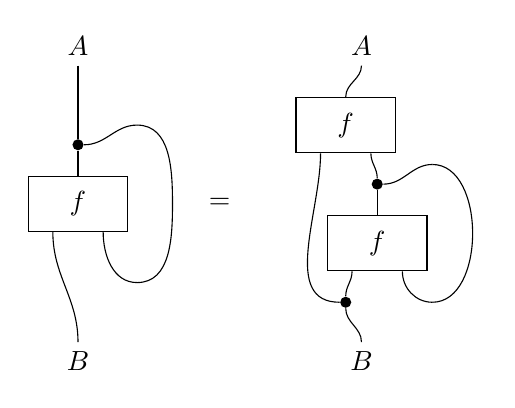
\begin{tikzpicture}
      \node[] (A) at (0, 2) {$A$};
      \node[box=1/0/2/0] (f) at (0, 0) {\quad f \quad};
      \node[] (B) at (0, -2) {$B$};
      \node[dot] (codiag) at (0, 0.75) {};
      \coordinate[] (C) at (1.2, 0) {};
      \coordinate[] (cup) at (0.75, -1) {};
      \coordinate[] (cap) at (0.75, 1) {};
      \node[] (eq) at (1.8, 0) {=};
      \node[] (Ad) at (3.6, 2) {$A$};
      \node[box=1/0/2/0] (fd1) at (3.4, 1) {\quad f \quad};
      \node[dot] (codiagd1) at (3.8, 0.25) {};
      \node[box=1/0/2/0] (fd2) at (3.8, -0.5) {\quad f \quad};
      \node[dot] (codiagd2) at (3.4, -1.25) {};
      \node[] (Bd) at (3.6, -2) {$B$};
      \coordinate[] (cupd) at (4.5, -1.25) {};
      \coordinate[] (capd) at (4.5, 0.5) {};
      \wires{
        A         = { south = codiag.north },
        f         = { south.1 = B, south.2 = cup.west },
        codiag    = { south = f.north, east = cap.west },
        C         = { south = cup.east, north = cap.east },
        Ad        = { south = fd1.north },
        fd1       = { south.1 = codiagd2.west, south.2 = codiagd1.north },
        codiagd1  = { south = fd2.north },
        fd2       = { south.1 = codiagd2.north, south.2 = cupd.west },
        codiagd2  = { south = Bd.north },
        cupd      = { east = capd.east },
        capd      = { west = codiagd1.east }, 
      }{}
    \end{tikzpicture}
    \caption{Fixpoint}
    \label{fig:fixpoint-string-diagram}
  \end{subfigure}%
  \begin{subfigure}{0.5\textwidth}
    \centering
    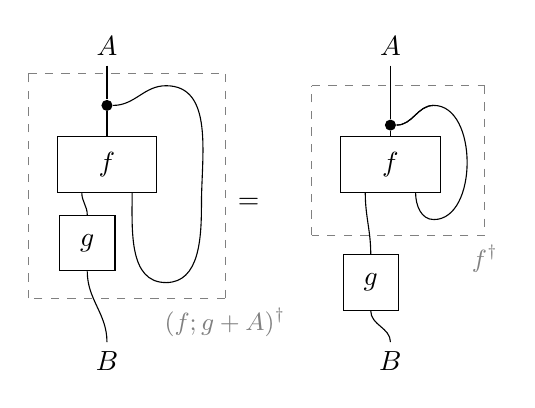
\begin{tikzpicture}
      \node[] (A) at (0, 2) {$A$};
      \node[box=1/0/2/0] (f) at (0, 0.5) {\quad f \quad};
      \node[box] (g) at (-0.25, -0.5) {g};
      \node[] (B) at (0, -2) {$B$};
      \node[dot] (codiag) at (0, 1.25) {};
      \coordinate[] (C) at (1.2, 0) {};
      \coordinate[] (cup) at (0.75, -1) {};
      \coordinate[] (cap) at (0.75, 1.5) {};
      \coordinate[] (box0) at (1.5, 1.65) {};
      \coordinate[label={[font=\small, text=gray]below:$(f;g + A)^\dagger$}] 
                    (box1) at (1.5, -1.2) {};
      \coordinate[] (box2) at (-1, -1.2) {};
      \coordinate[] (box3) at (-1, 1.65) {};
      \draw [gray, dashed] (box0) -- (box1);
      \draw [gray, dashed] (box1) -- (box2);
      \draw [gray, dashed] (box2) -- (box3);
      \draw [gray, dashed] (box3) -- (box0);
      \node[] (eq) at (1.8, 0) {=};
      \node[] (A2) at (3.6, 2) {$A$};
      \node[box=1/0/2/0] (f2) at (3.6, 0.5) {\quad f \quad};
      \node[box] (g2) at (3.35, -1) {g};
      \node[] (B2) at (3.6, -2) {$B$};
      \node[dot] (codiag2) at (3.6, 1) {};
      \coordinate[] (cup2) at (4.15, -0.2) {};
      \coordinate[] (cap2) at (4.15, 1.25) {};
      \coordinate[] (box02) at (4.8, 1.5) {};
      \coordinate[label={[font=\small, text=gray]below:$f^\dagger$}] 
                    (box12) at (4.8, -0.4) {};
      \coordinate[] (box22) at (2.6, -0.4) {};
      \coordinate[] (box32) at (2.6, 1.5) {};
      \draw [gray, dashed] (box02) -- (box12);
      \draw [gray, dashed] (box12) -- (box22);
      \draw [gray, dashed] (box22) -- (box32);
      \draw [gray, dashed] (box32) -- (box02);
      \wires{
        A         = { south = codiag.north },
        f         = { south.1 = g.north, south.2 = cup.west },
        g         = { south = B.north },
        codiag    = { south = f.north, east = cap.west },
        C         = { south = cup.east, north = cap.east },
        A2         = { south = codiag2.north },
        f2         = { south.1 = g2.north, south.2 = cup2.west },
        g2         = { south = B2.north },
        codiag2    = { south = f2.north, east = cap2.west },
        cup2       = { east = cap2.east },
        cap2       = { west = codiag2.east },
      }{}
    \end{tikzpicture}
    \caption{Naturality}
  \end{subfigure}
  \begin{subfigure}{0.5\textwidth}
    \centering
    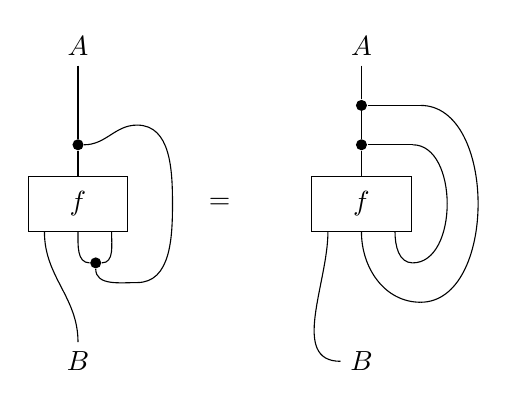
\begin{tikzpicture}
      \node[] (A) at (0, 2) {$A$};
      \node[box=1/0/3/0] (f) at (0, 0) {\quad f \quad};
      \node[] (B) at (0, -2) {$B$};
      \node[dot] (codiag) at (0, 0.75) {};
      \coordinate[] (C) at (1.2, 0) {};
      \coordinate[] (cup) at (0.75, -1) {};
      \coordinate[] (cap) at (0.75, 1) {};
      \node[dot] (codiag2) at (0.225, -0.75) {};
      \node[] (eq) at (1.8, 0) {=};
      \node[] (Ad) at (3.6, 2) {$A$};
      \node[box=1/0/3/0] (fd) at (3.6, 0) {\quad f \quad};
      \node[] (Bd) at (3.6, -2) {$B$};
      \node[dot] (codiagd) at (3.6, 1.25) {};
      \node[dot] (codiagd2) at (3.6, 0.75) {};
      \coordinate[] (Cd) at (4.8, 0) {};
      \coordinate[] (cupd) at (4.35, -1.25) {};
      \coordinate[] (capd) at (4.35, 1.25) {};
      \coordinate[] (cupd2) at (4.25, -0.75) {};
      \coordinate[] (capd2) at (4.25, 0.75) {};
      \wires{
        A         = { south = codiag.north },
        f         = { south.1 = B, south.2 = codiag2.west, south.3 = codiag2.east },
        codiag2   = { south = cup.west },
        codiag    = { south = f.north, east = cap.west },
        C         = { south = cup.east, north = cap.east },
        Ad        = { south = codiagd.north },
        codiagd   = { south = codiagd2.north, east = capd.west },
        codiagd2  = { south = fd.north, east = capd2.west },
        fd        = { south.1 = Bd, south.2 = cupd.west, south.3 = cupd2.west },
        cupd      = { east = capd.east },
        cupd2     = { east = capd2.east },
      }{}
    \end{tikzpicture}
    \caption{Codiagonal}
  \end{subfigure}%
  \begin{subfigure}{0.5\textwidth}
    \centering
    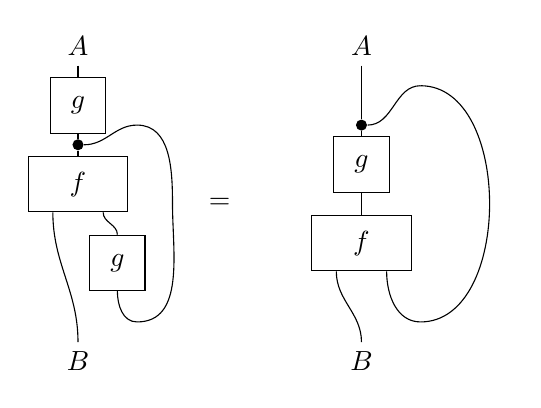
\begin{tikzpicture}
      \node[] (A) at (0, 2) {$A$};
      \node[box] (g) at (0, 1.25) {g};
      \node[box=1/0/2/0] (f) at (0, 0.25) {\quad f \quad};
      \node[] (B) at (0, -2) {$B$};
      \node[dot] (codiag) at (0, 0.75) {};
      \coordinate[] (C) at (1.2, 0) {};
      \coordinate[] (cup) at (0.75, -1.5) {};
      \coordinate[] (cap) at (0.75, 1) {};
      \node[box] (g2) at (0.5, -0.75) {g};
      \node[] (eq) at (1.8, 0) {=};
      \node[] (Ad) at (3.6, 2) {$A$};
      \node[box] (gd) at (3.6, 0.5) {g};
      \node[box=1/0/2/0] (fd) at (3.6, -0.5) {\quad f \quad};
      \node[] (Bd) at (3.6, -2) {$B$};
      \node[dot] (codiagd) at (3.6, 1) {};
      \coordinate[] (Cd) at (4.8, 0) {};
      \coordinate[] (cupd) at (4.35, -1.5) {};
      \coordinate[] (capd) at (4.35, 1.5) {};
      \wires{
        A         = { south = g.north },
        g         = { south = codiag.north },
        f         = { south.1 = B, south.2 = g2.north },
        g2        = { south = cup.west },
        codiag    = { south = f.north, east = cap.west },
        C         = { south = cup.east, north = cap.east },
        Ad        = { south = codiagd.north },
        codiagd   = { south = gd.north, east = capd.west },
        gd        = { south = fd.north },
        fd        = { south.1 = Bd, south.2 = cupd.west },
        cupd      = { east = capd.east },
      }{}
    \end{tikzpicture}
    \caption{Dinaturality}
  \end{subfigure}
  \caption{Representations of the Conway iteration axioms as string diagrams}
  \label{fig:elgot-ax-string-diagrams}
  \Description{Representations of the Conway iteration axioms as string diagrams}
\end{figure}

In particular, we note that naturality and codiagonal correspond directly to our rules
\brle{let-iter} and \brle{codiag} respectively; we will later see that dinaturality is derivable.

\TODO{explanation of strength in terms of captured variables; look at ML/Haskell again?}

We'd further like for our Conway iteration operator to play nicely with our premonoidal structure;
in particular, we require our Conway iteration operator to be \emph{strong}, defined as follows:
\begin{definition}[Strong Conway Iteration Operator]
  If $\mc{C}$ is distributive, we say an iteration operator $(\cdot)^\dagger$ is \emph{strong} if
  $$
  \forall f: A \to B + A, (C \otimes f ; \delta^{-1})^\dagger = C \otimes f^\dagger
  $$
\end{definition}

\TODO{effectful categories; centrality and purity}

\TODO{uniformity w.r.t effect system; note on derivability of dinaturality}

\TODO{\emph{general} models}

\TODO{models form a category; notion of morphism is obvious, see appendix}

\subsection{Semantics of \subiterexp{} Expressions}

\TODO{semantics; sentence per rule}

\begin{equation*}
  \dnt{A^q} = \dnt{\etoty{A^q}} \qquad
  !_{A^q} = !_{\etoty{A^q}} \qquad
  \Delta_{A^q} = \Delta_{\etoty{A^q}}
\end{equation*}

\begin{gather*}
  \boxed{\dnt{\Gamma^{\mb{q}}} : |\mc{C}|} \\
  \dnt{\cdot} = I
  \qquad \dnt{\Gamma^{\mb{q}}, x : A^q_\epsilon} 
          = \dnt{\Gamma^{\mb{q}}} \otimes \dnt{A^q}
\end{gather*}

\begin{figure}

  \begin{gather*}
    \dnt{\hasty{\Gamma^{\mb{q}}}{\epsilon}{\linl{a}}{A + B}}
    = \dnt{\hasty{\Gamma^{\mb{q}}}{\epsilon}{a}{A}} ; \iota_l \qquad
    \dnt{\hasty{\Gamma^{\mb{q}}}{\epsilon}{\linr{b}}{A + B}}
    = \dnt{\hasty{\Gamma^{\mb{q}}}{\epsilon}{b}{B}} ; \iota_r \\
    \dnt{\hasty{\Gamma^{\mb{q}}}{\epsilon}{\labort{a}}{A}}
    = \dnt{\hasty{\Gamma^{\mb{q}}}{\epsilon}{a}{\mb{0}}} ; 0_A
  \end{gather*}

  \begin{gather*}
    \boxed{\dnt{\cwk{\Gamma^{\mb{q}}}{\Delta^{\mb{q}'}_{\mb{e}'}}} 
      : \mc{C}_\bot(\dnt{\Gamma^{\mb{q}}}, \dnt{\Delta^{\mb{q}'}_{\mb{e}'}})} \\
    \dnt{\cwk{\cdot}{\cdot}} = \ms{id}_I \qquad
    \dnt{\cwk{\Gamma^{\mb{q}}, x : A^q_\epsilon}{\Delta^{\mb{q}'}_{\mb{e}'}}}
      = \dnt{\Gamma^{\mb{q}}} \otimes !_{A^q}
      ; \lambda
      ; \dnt{\cwk{\Gamma^{\mb{q}}}{\Delta^{\mb{q}'}_{\mb{e}'}}} \\
    \dnt{\cwk{\Gamma^{\mb{q}}, x : A^q_\epsilon}
              {\Delta^{\mb{q}'}_{\mb{e}'}, x : A^{q'}_{\epsilon'}}}
      = \dnt{\cwk{\Gamma^{\mb{q}}}{\Delta^{\mb{q}'}_{\mb{e}'}}} \otimes \begin{cases}
        \ms{id}_{\dnt{A}} & \text{if } q, q' \neq 0 \\
        !_{A^q} & \text{otherwise} \\
      \end{cases}
  \end{gather*}

  \begin{gather*}
    \boxed{\dnt{\qsp{\Gamma}{\mb{q}}{\mb{q}_l}{\mb{q}_r}} 
      : \mc{C}_\bot(\dnt{\Gamma^{\mb{q}}}, 
        \dnt{\Gamma^{\mb{q}_l}_{\mb{e}_l}} \otimes \dnt{\Gamma^{\mb{q}_r}_{\mb{e}_r}})} 
    \\
    \dnt{\qsp{\cdot}{\cdot}{\cdot}{\cdot}} = \rho^{-1}
    \\
    \dnt{\qsp{\Gamma, x : A}{(\mb{q}, q)}{(\mb{q}_l, q_l)}{(\mb{q}_r, q_r)}}
    = \dnt{\qsp{\Gamma}{\mb{q}}{\mb{q}_l}{\mb{q}_r}} \otimes
    \begin{cases}
      !_{A^q} ; \rho^{-1} & \text{if } q_l = q_r = 0 \text{ else} \\
      \lambda^{-1} & \text{if } q_l = 0 \text{ else} \\
      \rho^{-1} & \text{if } q_r = 0 \text{ else} \\
      \Delta_A & \text{otherwise}
    \end{cases} ; \sigma^{\ms{mid}}
  \end{gather*}
  \caption{Denotational semantics for structural \subiterexp{} judgements}
  \Description{}
\end{figure}

\begin{figure}
  \begin{gather*}
    \boxed{\dnt{\hasty{\Gamma^{\mb{q}}}{\epsilon}{a}{A}} 
      : \mc{C}_\epsilon(\dnt{\Gamma^{\mb{q}}}, \dnt{A})} \\
    \dnt{\hasty{\Gamma^{\mb{q}}}{\epsilon}{x}{A}} 
      = \dnt{\cwk{\Gamma^{\mb{q}}}{x : A^\oneq_\epsilon}}
    \qquad
    \dnt{\hasty{\Gamma^{\mb{q}}}{\epsilon}{f\;a}{B}} 
      = \dnt{\hasty{\Gamma^{\mb{q}}}{\epsilon}{a}{A}} ; \dnt{f} \\
    \dnt{\hasty{\Gamma^{\mb{q}}}{\epsilon}{\letexpr{x}{a}{b}}{B}} 
      = \dnt{\qsp{\Gamma}{\mb{q}}{\mb{q}_l}{\mb{q}_r}}
      ; \dnt{\Gamma^{\mb{q}_l}} 
        \otimes \dnt{\hasty{\Gamma^{\mb{q}_r}}{\epsilon}{a}{A}}
      ; \dnt{\hasty{\Gamma^{\mb{q}_l}, x : A}{\epsilon}{b}{B}}
    \\
    \dnt{\hasty{\Gamma^{\mb{q}}}{\epsilon}{()}{\mb{1}}}
      = \dnt{\cwk{\Gamma^{\mb{q}}}{\cdot}}
    \\
    \dnt{\hasty{\Gamma^{\mb{q}}}{\epsilon}{(a, b)}{A \otimes B}}
      = \dnt{\qsp{\Gamma}{\mb{q}}{\mb{q}_l}{\mb{q}_r}}
      ; \dnt{\hasty{\Gamma^{\mb{q}_l}}{\epsilon}{a}{A}}
      \otimes \dnt{\hasty{\Gamma^{\mb{q}_r}}{\epsilon}{b}{B}}
  \end{gather*}
  \begin{align*}
    \dnt{\hasty{\Gamma^{\mb{q}}}{\epsilon}{\letexpr{(x, y)}{a}{c}}{C}}
    = & \; \dnt{\qsp{\Gamma}{\mb{q}}{\mb{q}_l}{\mb{q}_r}}
      ; \dnt{\Gamma^{\mb{q}_l}}
      \otimes \dnt{\hasty{\Gamma^{\mb{q}_r}}{\epsilon}{a}{A \otimes B}}
    \\ & 
    ; \alpha_{\Gamma^{\mb{q}_r} \otimes A \otimes B}
    ; \dnt{\hasty{\Gamma^{\mb{q}_l}, x : A, y : B}{\epsilon}{c}{C}} \\
  \end{align*}
  \begin{align*}
    \dnt{\hasty{\Gamma^{\mb{q}}}{\epsilon}{\caseexpr{e}{x}{a}{y}{b}}{C}}
    =& \; 
    \dnt{\qsp{\Gamma}{\mb{q}}{\mb{q}_l}{\mb{q}_r}}
    ; \dnt{\Gamma^{\mb{q}_l}} 
    \otimes \dnt{\hasty{\Gamma^{\mb{q}_r}}{\epsilon}{e}{A + B}}
    ; \delta^{-1} \\ & 
    ; [
      \dnt{\hasty{\Gamma^{\mb{q}_l}, x : A}{\epsilon}{a}{C}},
      \dnt{\hasty{\Gamma^{\mb{q}_l}, y : B}{\epsilon}{b}{C}}
    ]
  \end{align*}
  \begin{align*}
    \dnt{\hasty{\Gamma^{\mb{q}}}{\epsilon}{\liter{a}{x}{b}}{B}}
    &= 
    \dnt{\qsp{\Gamma}{\mb{q}}{\mb{q}_l}{\mb{q}_r}}
    ; \dnt{\Gamma^{\mb{q}_l}}
      \otimes \dnt{\hasty{\Gamma^{\mb{q}_r}}{\epsilon}{a}{A}} \\ &
    ; (
      \dnt{\qsp{\Gamma}{\mb{q}_l}{\mb{q}_l}{\mb{q}_l}} \otimes \dnt{A} 
      ; \alpha
      ; \dnt{\Gamma^{\mb{q}_l}} 
        \otimes \dnt{\hasty{\Gamma^{\mb{q}_r}, x : A}{\epsilon}{b}{B + A}}
      ; \delta^{-1}
    )^\dagger \\ &
    ; \dnt{\cwk{\Gamma^{\mb{q}_l}}{\cdot}} \otimes \dnt{B}
    ; \rho
  \end{align*}
  \caption{Denotational semantics for \subiterexp{} expressions}
  \Description{}
\end{figure}

\TODO{coherence text}

\begin{lemma}[Coherence]
  Given derivations $D$ for $\hasty{\Gamma^{\mb{q}}}{\epsilon}{a}{A}$ and $D'$ for
  $\hasty{\Gamma^{\mb{q}}}{\epsilon'}{a}{A}$, we have $\dnt{D} = \dnt{D'}$
\end{lemma}

\TODO{therefore, $\dnt{\ms{stmt}}$ notation is justified, and non-effect notation is justified}

\begin{lemma}[Weakening]
  Given $\cwk{\Gamma^{\mb{q}}}{\Delta^{\mb{q}'}}$ and
  $\hasty{\Delta^{\mb{q}'}}{\epsilon}{a}{A}$, we have that
  $$
  \dnt{\cwk{\Gamma^{\mb{q}}}{\Delta^{\mb{q}'}}} ; \dnt{\hasty{\Delta^{\mb{q}'}}{\epsilon}{a}{A}}
  = \dnt{\hasty{\Gamma^{\mb{q}}}{\epsilon}{a}{A}}
  $$
\end{lemma}

\subsection{Substitution}

\TODO{semantics of substitution}

\begin{theorem}[Soundness of Substitution]
  Given $\issubst{\Gamma^{\mb{q}}}{\eta}{\sigma}{\Delta^{\mb{q'}}}$ and
  $\hasty{\Delta^{\mb{q}'}}{\epsilon}{a}{A}$, we have
  \begin{align*}
  \eta \rightmove \epsilon \implies
  \dnt{\issubst{\Gamma^{\mb{q}}}{\eta}{\sigma}{\Delta^{\mb{q'}}}} 
    ; \dnt{\hasty{\Delta^{\mb{q}'}}{\epsilon}{a}{A}}
  \leq \dnt{\hasty{\Gamma^{\mb{q}}}{}{[\sigma]a}{A}} \\
  \eta \leftmove \epsilon \implies
  \dnt{\issubst{\Gamma^{\mb{q}}}{\eta}{\sigma}{\Delta^{\mb{q'}}}} 
    ; \dnt{\hasty{\Delta^{\mb{q}'}}{\epsilon}{a}{A}}
  \geq \dnt{\hasty{\Gamma^{\mb{q}}}{}{[\sigma]a}{A}}
  \end{align*}
\end{theorem}

\subsection{Soundness}

\begin{definition}
  We say a model $\mc{M}$ \emph{validates} a typed refinement family $\mc{R}$, written $\mc{M}
  \models \mc{R}$, if, for all
  $
  (\tmle{\Gamma^{\mb{q}}}{}{a}{b}{A}) \in \mc{R}
  $
  we have that
  $
  \dnt{\hasty{\Gamma}{\epsilon}{a}{A}} \leq \dnt{\hasty{\Gamma}{\epsilon}{b}{A}}
  $
\end{definition}

\TODO{wide subcategory $\ms{Mod}(\mc{R}) \subseteq \ms{Mod}(\mc{S})$ of models \emph{w.r.t.} a
specific refinement relation $\mc{R}$}

\TODO{this forms a lattice, yo, with bottom element $\mc{R} = \varnothing$}

\begin{theorem}[Soundness]
  If $\mc{M} \models \mc{R}$, given $\tmle{\Gamma^{\mb{q}}}{\mc{R}}{a}{b}{A}$, we have
  $\dnt{\hasty{\Gamma}{\epsilon}{a}{A}}_{\mc{M}} \leq \dnt{\hasty{\Gamma}{\epsilon}{b}{A}}_{\mc{M}}$
  . In particular, this implies that $\mc{M} \models \mc{R} \iff \mc{M} \models \ms{Th}(\mc{R})$.
\end{theorem}

\subsection{Syntactic Models and Completeness}

\TODO{define $\ms{Tm}(\mc{R})$}

\begin{theorem}[Completeness]
  If $\dnt{\hasty{\Gamma}{}{a}{A}}_{\ms{Tm}(\mc{R})} \leq
  \dnt{\hasty{\Gamma}{}{b}{A}}_{\ms{Tm}(\mc{R})}$, then
  $
  \tmle{\Gamma}{\mc{R}}{a}{b}{A}
  $. In particular, the following are equivalent:
  \begin{enumerate}
    \item $\dnt{\hasty{\Gamma}{}{a}{A}}_{\ms{Tm}(\mc{R})} \leq
    \dnt{\hasty{\Gamma}{}{b}{A}}_{\ms{Tm}(\mc{R})}$
    \item $\tmle{\Gamma}{\mc{R}}{a}{b}{A}$
    \item $\forall \mc{M} \models \mc{R}, \dnt{\hasty{\Gamma}{}{a}{A}}_{\mc{M}} \leq
    \dnt{\hasty{\Gamma}{}{b}{A}}_{\mc{M}}$
  \end{enumerate}
\end{theorem}

\TODO{or, in more categorical language, $\ms{Tm}(\mc{R})$ is the initial object of
$\ms{Mod}(\mc{R})$.}

\section{SSA Typing and Semantics}

\TODO{introduce judgement and label contexts}

\TODO{typing rules go brr; explain where rec/nonrec; nonrec can always be promoted to rec at an
iterative effect}

\TODO{denotational semantics}

\TODO{by completeness, $\subseteq$ expressions; this is like \citet{bohm-jacopini}}

\TODO{by translation, expressions $\subseteq$; translation procedure goes to appendix}

\section{Concrete Models}

\TODO{UB and printing}

\TODO{separation logic}

\TODO{Release-Acquire Weak Memory}

\section{Discussion and Related Work}

\TODO{this}

\subsection*{Acknowledgements}

This work was supported in part by a European Research Council (ERC) Consolidator Grant for the
project ``TypeFoundry'', funded under the European Union's Horizon 2020 Framework Programme (grant
agreement no. 101002277).

\bibliographystyle{ACM-Reference-Format}
\bibliography{references}

\clearpage 

\appendix

\end{document}
\endinput
